\documentclass[dvips, 10pt]{article}
\usepackage{graphicx}
\usepackage{rotating}
\setlength{\oddsidemargin}{-0.45in}
\setlength{\evensidemargin}{-0.45in}
\setlength{\textwidth}{7.0in}
\setlength{\topmargin}{-0.70in}
\setlength{\textheight}{9.5in}
\pagestyle{myheadings}
\markright{ {\rm {
GLND DSMB Report-Recruitment, Baseline, and Follow-up OPEN SESSION
 \hspace{2em}
Wed Apr 13 11:52:35 EDT 2011
\hfill
\hspace{3em}
}}}
\headsep=0.2in
\begin{document}
\vspace*{1in}
\begin{center}
{\Huge{CONFIDENTIAL}}
\end{center}
\vspace*{0.5in}
\begin{center}
{\Huge{Efficacy and Mechanisms of GLN Dipeptide in the SICU GLND Trial}}
\end{center}
\vspace*{0.5in}
\begin{center}
{\Huge{Data Safety Monitoring Board Report}}
\end{center}
\vspace*{0.25in}
\begin{center}
{\Huge{
Recruitment, Baseline, and Follow-up  OPEN SESSION
}}
\end{center}
\vspace*{1in}
\begin{center}
{\Huge{GLND DSMB Meeting}}
\end{center}
\begin{center}
{\Huge{
May 3, 2011
}}
\end{center}
\begin{center}
{\Huge{10am-2pm EDT}}
\end{center}
\vspace*{1in}
\begin{center}
\noindent
{\Large{Includes patients enrolled and follow-up data received as of April 4, 2011}}
\end{center}
\vspace*{0.5in}
\begin{center}
{\Large{Report prepared  Wed Apr 13 11:52:35 EDT 2011 }}
\end{center}
\clearpage
\vspace*{1in}
\begin{center}
{\Huge{Table of Contents}}
\end{center}
\listoftables
\listoffigures
\clearpage
\begin{table}[t]
\caption
{ Patient Screening and Enrollment. }
\begin{center}
\begin{tabular}{ @{}l@{}
@{}l@{}@{}p{1.5em}@{}@{}c@{}@{}p{1.5em}@{}@{}c@{}@{}p{1.5em}@{}@{}c@{}@{}p{1.5em}@{}@{}c@{}
}
\hline

& \parbox{6em}{\begin{center}Clinical Center\end{center}} && \parbox{6em}{\begin{center}No. Screened\end{center}} && \parbox{6em}{\begin{center}No. Eligible (\%)\end{center}} && \parbox{6em}{\begin{center}No. Enrolled (\%)\end{center}} && \parbox{6em}{\begin{center}Date IRB Approved\end{center}} \\

\hline

\\
& Emory && 461 && 78 ( 17\%) && 55 ( 71\%) && 11/01/06 \\
& Miriam && 51 && 22 ( 43\%) && 9 ( 41\%) && 01/01/07 \\
& Vanderbilt && 358 && 62 ( 17\%) && 38 ( 61\%) && 01/01/07 \\
& Colorado && 163 && 36 ( 22\%) && 33 ( 92\%) && 02/01/07 \\
& Wisconsin && 87 && 9 ( 10\%) && 5 ( 56\%) && 11/02/09 \\
& Total && 1120 && 207 ( 18\%) && 140 ( 68\%) && . \\
\\
\hline \\

\end{tabular}

\end{center}
 \end{table}
\begin{table}[t]
\caption
{ Recruitment in the last 6 months. }
\begin{center}
\begin{tabular}{ @{}l@{}
@{}c@{}@{}p{1.5em}@{}@{}c@{}@{}p{1.5em}@{}@{}c@{}
}
\hline

& \parbox{6em}{\begin{center}Month\end{center}} && \parbox{6em}{\begin{center}Patients Recruited\end{center}} && \parbox{6em}{\begin{center}Total Recruited\end{center}} \\

\hline

\\
& OCT10 && 0 && 130 \\
& NOV10 && 1 && 131 \\
& DEC10 && 0 && 131 \\
& JAN11 && 4 && 135 \\
& FEB11 && 3 && 138 \\
& MAR11 && 3 && 141 \\
\\
\hline \\

\end{tabular}

\end{center}
 \end{table}

\begin{figure}
\resizebox{6.5in}{!}{\rotatebox{90}{\includegraphics{//glnd//sas//reporting//recruitment.ps}}}
\caption{Recruitment Projections}
\end{figure}

\begin{figure}
\resizebox{6.5in}{!}{\rotatebox{0}{\includegraphics{//glnd//sas//reporting//rc13.ps}}}
\caption{Recruitment Projections by Center}
\end{figure}
\clearpage

\begin{figure}
\resizebox{6.5in}{!}{\rotatebox{0}{\includegraphics{//glnd//sas//reporting//rc45.ps}}}
\caption{Recruitment Projections by Center (continued)}
\end{figure}
\clearpage
\begin{table}[t]
\caption
{ Patient Screening and Enrollment Within Last 6 months. }
\begin{center}
\begin{tabular}{ @{}l@{}
@{}l@{}@{}p{1.5em}@{}@{}c@{}@{}p{1.5em}@{}@{}c@{}@{}p{1.5em}@{}@{}c@{}@{}p{1.5em}@{}@{}c@{}
}
\hline

& \parbox{6em}{\begin{center}Month\end{center}} && \parbox{6em}{\begin{center}Clinical Center\end{center}} && \parbox{6em}{\begin{center}No. Screened\end{center}} && \parbox{6em}{\begin{center}No. Eligible (\%)\end{center}} && \parbox{6em}{\begin{center}No. Enrolled (\%)\end{center}} \\

\hline

\\
& OCT2010 && Emory && 8 && 0 (  0\%) && - \\
&  && Vanderbilt && 3 && 0 (  0\%) && - \\
&  && Colorado && 0 && - && - \\
&  && Wisconsin && 2 && 0 (  0\%) && - \\
&  && Total && 13 && 0 (  0\%) && - \\
&  &&  &&  &&  &&  \\
& NOV2010 && Emory && 12 && 2 ( 17\%) && 0 (  0\%) \\
&  && Vanderbilt && 4 && 1 ( 25\%) && 0 (  0\%) \\
&  && Colorado && 0 && - && - \\
&  && Wisconsin && 7 && 1 ( 14\%) && 1 (100\%) \\
&  && Total && 23 && 4 ( 17\%) && 1 ( 25\%) \\
&  &&  &&  &&  &&  \\
& DEC2010 && Emory && 8 && 0 (  0\%) && - \\
&  && Vanderbilt && 5 && 1 ( 20\%) && 0 (  0\%) \\
&  && Colorado && 0 && - && - \\
&  && Wisconsin && 7 && 1 ( 14\%) && 0 (  0\%) \\
&  && Total && 20 && 2 ( 10\%) && 0 (  0\%) \\
&  &&  &&  &&  &&  \\
& JAN2011 && Emory && 13 && 4 ( 31\%) && 3 ( 75\%) \\
&  && Vanderbilt && 9 && 1 ( 11\%) && 1 (100\%) \\
&  && Colorado && 1 && 0 (  0\%) && - \\
&  && Wisconsin && 8 && 0 (  0\%) && - \\
&  && Total && 31 && 5 ( 16\%) && 4 ( 80\%) \\
&  &&  &&  &&  &&  \\
& FEB2011 && Emory && 8 && 1 ( 13\%) && 1 (100\%) \\
&  && Vanderbilt && 8 && 3 ( 38\%) && 2 ( 67\%) \\
&  && Colorado && 0 && - && - \\
&  && Wisconsin && 2 && 0 (  0\%) && - \\
&  && Total && 18 && 4 ( 22\%) && 3 ( 75\%) \\
&  &&  &&  &&  &&  \\
& MAR2011 && Emory && 7 && 1 ( 14\%) && 0 (  0\%) \\
&  && Vanderbilt && 9 && 2 ( 22\%) && 1 ( 50\%) \\
&  && Colorado && 1 && 1 (100\%) && 1 (100\%) \\
&  && Wisconsin && 3 && 0 (  0\%) && - \\
&  && Total && 20 && 4 ( 20\%) && 2 ( 50\%) \\
&  &&  &&  &&  &&  \\
\\
\hline \\

\end{tabular}

\end{center}
 \end{table}
\begin{table}[tbp]
\caption
{ Reasons Patients Were Ineligible at Screening - Emory. }
\begin{center}
\begin{tabular}{ @{}l@{}
@{}c@{}
}
\hline

& \parbox{6em}{\begin{center}Total\end{center}} \\
 & n=472 \\
 \cline{2-2} 
 Characteristic &
 \makebox[1.5em]{n}\makebox[3.5em][r]{(\%)} \\
 \hline
\\
\parbox[b]{ 70mm }{\raggedright{{\bf Reason Not Eligible }}} &
  \\
 \hspace{1em} AGE not 18-80 &
 \makebox[1.5em][r]{6}\makebox[3.5em][r]{(1.3)} \\
 \hspace{1em} BMI $ \ge $ 40 &
 \makebox[1.5em][r]{33}\makebox[3.5em][r]{(7.0)} \\
 \hspace{1em} Burn Trauma Injury &
 \makebox[1.5em][r]{3}\makebox[3.5em][r]{(0.6)} \\
 \hspace{1em} Central Venous PN $<$ 7 days &
 \makebox[1.5em][r]{2}\makebox[3.5em][r]{(0.4)} \\
 \hspace{1em} Cirrhosis or Bilirubin $ \ge $10 &
 \makebox[1.5em][r]{29}\makebox[3.5em][r]{(6.1)} \\
 \hspace{1em} Clinical Sepsis within 24 hrs study entry &
 \makebox[1.5em][r]{7}\makebox[3.5em][r]{(1.5)} \\
 \hspace{1em} Ent/Parent Feedings &
 \makebox[1.5em][r]{24}\makebox[3.5em][r]{(5.1)} \\
 \hspace{1em} Gastric Surgery or Whipple &
 \makebox[1.5em][r]{11}\makebox[3.5em][r]{(2.3)} \\
 \hspace{1em} History of HIV/AIDS &
 \makebox[1.5em][r]{4}\makebox[3.5em][r]{(0.8)} \\
 \hspace{1em} Malignancy &
 \makebox[1.5em][r]{105}\makebox[3.5em][r]{(22.2)} \\
 \hspace{1em} NOT in Post Op Days Range &
 \makebox[1.5em][r]{58}\makebox[3.5em][r]{(12.3)} \\
 \hspace{1em} No Central Access &
 \makebox[1.5em][r]{14}\makebox[3.5em][r]{(3.0)} \\
 \hspace{1em} Organ Transplant &
 \makebox[1.5em][r]{23}\makebox[3.5em][r]{(4.9)} \\
 \hspace{1em} Received Investigational Drug &
 \makebox[1.5em][r]{19}\makebox[3.5em][r]{(4.0)} \\
 \hspace{1em} Received PN 4+ days &
 \makebox[1.5em][r]{2}\makebox[3.5em][r]{(0.4)} \\
 \hspace{1em} Renal Dysfunction &
 \makebox[1.5em][r]{93}\makebox[3.5em][r]{(19.7)} \\
 \hspace{1em} Require PN$<$7 days &
 \makebox[1.5em][r]{15}\makebox[3.5em][r]{(3.2)} \\
 \hspace{1em} Seizure Hist/Disorder &
 \makebox[1.5em][r]{20}\makebox[3.5em][r]{(4.2)} \\
 \hspace{1em} Unexplained Encephalopathy &
 \makebox[1.5em][r]{4}\makebox[3.5em][r]{(0.8)} \\
 \vspace{0em} \\
\hline \\ 
\end{tabular}

\parbox{ 5in }{ *n represents total number of reasons given for ineligible patients } \\
 \vspace{1em}\end{center}
 \end{table}
\begin{table}[tbp]
\caption
{ Reasons Patients Were Ineligible at Screening - Vanderbilt. }
\begin{center}
\begin{tabular}{ @{}l@{}
@{}c@{}
}
\hline

& \parbox{6em}{\begin{center}Total\end{center}} \\
 & n=346 \\
 \cline{2-2} 
 Characteristic &
 \makebox[1.5em]{n}\makebox[3.5em][r]{(\%)} \\
 \hline
\\
\parbox[b]{ 70mm }{\raggedright{{\bf Reason Not Eligible }}} &
  \\
 \hspace{1em} AGE not 18-80 &
 \makebox[1.5em][r]{4}\makebox[3.5em][r]{(1.2)} \\
 \hspace{1em} BMI $ \ge $ 40 &
 \makebox[1.5em][r]{44}\makebox[3.5em][r]{(12.7)} \\
 \hspace{1em} Burn Trauma Injury &
 \makebox[1.5em][r]{5}\makebox[3.5em][r]{(1.4)} \\
 \hspace{1em} Central Venous PN $<$ 7 days &
 \makebox[1.5em][r]{11}\makebox[3.5em][r]{(3.2)} \\
 \hspace{1em} Cirrhosis or Bilirubin $ \ge $10 &
 \makebox[1.5em][r]{11}\makebox[3.5em][r]{(3.2)} \\
 \hspace{1em} Clinical Sepsis within 24 hrs study entry &
 \makebox[1.5em][r]{20}\makebox[3.5em][r]{(5.8)} \\
 \hspace{1em} Ent/Parent Feedings &
 \makebox[1.5em][r]{14}\makebox[3.5em][r]{(4.0)} \\
 \hspace{1em} Gastric Surgery or Whipple &
 \makebox[1.5em][r]{5}\makebox[3.5em][r]{(1.4)} \\
 \hspace{1em} In SICU due to wrong reason &
 \makebox[1.5em][r]{27}\makebox[3.5em][r]{(7.8)} \\
 \hspace{1em} Malignancy &
 \makebox[1.5em][r]{85}\makebox[3.5em][r]{(24.6)} \\
 \hspace{1em} NOT in Post Op Days Range &
 \makebox[1.5em][r]{20}\makebox[3.5em][r]{(5.8)} \\
 \hspace{1em} Organ Transplant &
 \makebox[1.5em][r]{12}\makebox[3.5em][r]{(3.5)} \\
 \hspace{1em} Physician(s) Will NOT Allow &
 \makebox[1.5em][r]{1}\makebox[3.5em][r]{(0.3)} \\
 \hspace{1em} Received Investigational Drug &
 \makebox[1.5em][r]{2}\makebox[3.5em][r]{(0.6)} \\
 \hspace{1em} Received PN 4+ days &
 \makebox[1.5em][r]{1}\makebox[3.5em][r]{(0.3)} \\
 \hspace{1em} Renal Dysfunction &
 \makebox[1.5em][r]{41}\makebox[3.5em][r]{(11.8)} \\
 \hspace{1em} Require PN$<$7 days &
 \makebox[1.5em][r]{23}\makebox[3.5em][r]{(6.6)} \\
 \hspace{1em} Seizure Hist/Disorder &
 \makebox[1.5em][r]{19}\makebox[3.5em][r]{(5.5)} \\
 \hspace{1em} Unexplained Encephalopathy &
 \makebox[1.5em][r]{1}\makebox[3.5em][r]{(0.3)} \\
 \vspace{0em} \\
\hline \\ 
\end{tabular}
\end{center}
 \end{table}
\begin{table}[tbp]
\caption
{ Reasons Patients Were Ineligible at Screening - Colorado. }
\begin{center}
\begin{tabular}{ @{}l@{}
@{}c@{}
}
\hline

& \parbox{6em}{\begin{center}Total\end{center}} \\
 & n=162 \\
 \cline{2-2} 
 Characteristic &
 \makebox[1.5em]{n}\makebox[3.5em][r]{(\%)} \\
 \hline
\\
\parbox[b]{ 70mm }{\raggedright{{\bf Reason Not Eligible }}} &
  \\
 \hspace{1em} AGE not 18-80 &
 \makebox[1.5em][r]{1}\makebox[3.5em][r]{(0.6)} \\
 \hspace{1em} BMI $ \ge $ 40 &
 \makebox[1.5em][r]{6}\makebox[3.5em][r]{(3.7)} \\
 \hspace{1em} Burn Trauma Injury &
 \makebox[1.5em][r]{1}\makebox[3.5em][r]{(0.6)} \\
 \hspace{1em} Central Venous PN $<$ 7 days &
 \makebox[1.5em][r]{2}\makebox[3.5em][r]{(1.2)} \\
 \hspace{1em} Cirrhosis or Bilirubin $ \ge $10 &
 \makebox[1.5em][r]{17}\makebox[3.5em][r]{(10.5)} \\
 \hspace{1em} Clinical Sepsis within 24 hrs study entry &
 \makebox[1.5em][r]{2}\makebox[3.5em][r]{(1.2)} \\
 \hspace{1em} Ent/Parent Feedings &
 \makebox[1.5em][r]{2}\makebox[3.5em][r]{(1.2)} \\
 \hspace{1em} Gastric Surgery or Whipple &
 \makebox[1.5em][r]{7}\makebox[3.5em][r]{(4.3)} \\
 \hspace{1em} History of HIV/AIDS &
 \makebox[1.5em][r]{2}\makebox[3.5em][r]{(1.2)} \\
 \hspace{1em} In SICU due to wrong reason &
 \makebox[1.5em][r]{2}\makebox[3.5em][r]{(1.2)} \\
 \hspace{1em} Malignancy &
 \makebox[1.5em][r]{74}\makebox[3.5em][r]{(45.7)} \\
 \hspace{1em} NOT in Post Op Days Range &
 \makebox[1.5em][r]{4}\makebox[3.5em][r]{(2.5)} \\
 \hspace{1em} Organ Transplant &
 \makebox[1.5em][r]{10}\makebox[3.5em][r]{(6.2)} \\
 \hspace{1em} Patient Pregnant &
 \makebox[1.5em][r]{1}\makebox[3.5em][r]{(0.6)} \\
 \hspace{1em} Physician(s) Will NOT Allow &
 \makebox[1.5em][r]{4}\makebox[3.5em][r]{(2.5)} \\
 \hspace{1em} Received Investigational Drug &
 \makebox[1.5em][r]{2}\makebox[3.5em][r]{(1.2)} \\
 \hspace{1em} Received PN 4+ days &
 \makebox[1.5em][r]{1}\makebox[3.5em][r]{(0.6)} \\
 \hspace{1em} Renal Dysfunction &
 \makebox[1.5em][r]{14}\makebox[3.5em][r]{(8.6)} \\
 \hspace{1em} Require PN$<$7 days &
 \makebox[1.5em][r]{2}\makebox[3.5em][r]{(1.2)} \\
 \hspace{1em} Seizure Hist/Disorder &
 \makebox[1.5em][r]{7}\makebox[3.5em][r]{(4.3)} \\
 \hspace{1em} Unexplained Encephalopathy &
 \makebox[1.5em][r]{1}\makebox[3.5em][r]{(0.6)} \\
 \vspace{0em} \\
\hline \\ 
\end{tabular}
\end{center}
 \end{table}
\begin{table}[tbp]
\caption
{ Reasons Patients Were Ineligible at Screening - Wisconsin. }
\begin{center}
\begin{tabular}{ @{}l@{}
@{}c@{}
}
\hline

& \parbox{6em}{\begin{center}Total\end{center}} \\
 & n=104 \\
 \cline{2-2} 
 Characteristic &
 \makebox[1.5em]{n}\makebox[3.5em][r]{(\%)} \\
 \hline
\\
\parbox[b]{ 70mm }{\raggedright{{\bf Reason Not Eligible }}} &
  \\
 \hspace{1em} AGE not 18-80 &
 \makebox[1.5em][r]{3}\makebox[3.5em][r]{(2.9)} \\
 \hspace{1em} BMI $ \ge $ 40 &
 \makebox[1.5em][r]{13}\makebox[3.5em][r]{(12.5)} \\
 \hspace{1em} Burn Trauma Injury &
 \makebox[1.5em][r]{2}\makebox[3.5em][r]{(1.9)} \\
 \hspace{1em} Cirrhosis or Bilirubin $ \ge $10 &
 \makebox[1.5em][r]{11}\makebox[3.5em][r]{(10.6)} \\
 \hspace{1em} Clinical Sepsis within 24 hrs study entry &
 \makebox[1.5em][r]{6}\makebox[3.5em][r]{(5.8)} \\
 \hspace{1em} Ent/Parent Feedings &
 \makebox[1.5em][r]{1}\makebox[3.5em][r]{(1.0)} \\
 \hspace{1em} Malignancy &
 \makebox[1.5em][r]{32}\makebox[3.5em][r]{(30.8)} \\
 \hspace{1em} Organ Transplant &
 \makebox[1.5em][r]{8}\makebox[3.5em][r]{(7.7)} \\
 \hspace{1em} Physician(s) Will NOT Allow &
 \makebox[1.5em][r]{2}\makebox[3.5em][r]{(1.9)} \\
 \hspace{1em} Renal Dysfunction &
 \makebox[1.5em][r]{18}\makebox[3.5em][r]{(17.3)} \\
 \hspace{1em} Require PN$<$7 days &
 \makebox[1.5em][r]{2}\makebox[3.5em][r]{(1.9)} \\
 \hspace{1em} Seizure Hist/Disorder &
 \makebox[1.5em][r]{3}\makebox[3.5em][r]{(2.9)} \\
 \hspace{1em} Unexplained Encephalopathy &
 \makebox[1.5em][r]{3}\makebox[3.5em][r]{(2.9)} \\
 \vspace{0em} \\
\hline \\ 
\end{tabular}
\end{center}
 \end{table}
\clearpage
\begin{table}[t]
\caption
{ Reasons Patients Eligible at Screening Were Not Enrolled. }
\begin{center}
\begin{tabular}{ @{}l@{}
@{}l@{}@{}p{1.5em}@{}@{}c@{}@{}p{1.5em}@{}@{}l@{}
}
\hline

& \parbox{6em}{\begin{center}Clinical Center\end{center}} && \parbox{6em}{\begin{center}GLND ID No.\end{center}} && \parbox{6em}{\begin{center}Reason Not Enrolled\end{center}} \\

\hline

\\
& Emory && 19042 && By time family's assent received, subject was to be sent to \\
& Emory && 19047 && Patient did not wish to participate \\
& Emory && 19049 && Patient screened on holiday, DCC unavailable to randomize \\
& Emory && 19065 && Patient did not wish to participate \\
& Emory && 19077 && Patient Death \\
& Emory && 19080 && Patient did not wish to participate \\
& Emory && 19092 && patients family did not want to participate \\
& Emory && 19103 && Patient's wife felt that patient had already been through al \\
& Emory && 19105 && By the time PN would be hung, patient would no longer be in \\
& Emory && 19107 && no family member lar to give consent \\
& Emory && 19108 && patient family did not want to participate \\
& Emory && 19111 && no family member available to consent \\
& Emory && 19174 && Family did not want to participate \\
& Emory && 19176 && Patient did not wish to participate \\
& Emory && 19194 && Patient Death \\
& Emory && 19216 && Patient Death \\
& Emory && 19340 && Patient did not wish to participate \\
& Emory && 19367 && Patient did not wish to participate \\
& Emory && 19391 && Patient did not wish to participate \\
& Emory && 19415 && Patient refused as she wouldn't get paid \\
& Emory && 19418 && Patient did not wish to participate \\
& Emory && 19442 && Patient did not wish to participate \\
& Emory && 19458 && Patient did not wish to participate \\
\\
\hline \\

\end{tabular}

\end{center}
 \end{table}
\begin{table}[t]
\caption
{ Reasons Patients Eligible at Screening Were Not Enrolled (continued). }
\begin{center}
\begin{tabular}{ @{}l@{}
@{}l@{}@{}p{1.5em}@{}@{}c@{}@{}p{1.5em}@{}@{}l@{}
}
\hline

& \parbox{6em}{\begin{center}Clinical Center\end{center}} && \parbox{6em}{\begin{center}GLND ID No.\end{center}} && \parbox{6em}{\begin{center}Reason Not Enrolled\end{center}} \\

\hline

\\
& Vanderbilt && 39002 && Unable or Unwilling to Participate \\
& Vanderbilt && 39006 && Site randomized as 32006 without pt consent; all CRF images \\
& Vanderbilt && 39007 && Patient did not wish to participate \\
& Vanderbilt && 39013 && Patient did not wish to participate \\
& Vanderbilt && 39023 && Pt. unable to consent; No LAR/immediate fam. \\
& Vanderbilt && 39024 && Non-English speaking (secondary to the code of Federal Regul \\
& Vanderbilt && 39041 && Pt. is non-English speaking \\
& Vanderbilt && 39073 && patient mentally handicapped \& withough available surrogate \\
& Vanderbilt && 39080 && patient intubated and sedated; family unavailable for surrog \\
& Vanderbilt && 39098 && family refuses consent \\
& Vanderbilt && 39105 && Plan to withdraw life support \\
& Vanderbilt && 39126 && Unable or Unwilling to Participate \\
& Vanderbilt && 39136 && imminent death \\
& Vanderbilt && 39139 && Iniminent Death \\
& Vanderbilt && 39210 && Family unavailable -$>$ none \\
& Vanderbilt && 39225 && No consulting party available \\
& Vanderbilt && 39227 && Unable or Unwilling to Participate \\
& Vanderbilt && 39228 && Patient did not wish to participate \\
& Vanderbilt && 39232 && Patient did not wish to participate \\
& Vanderbilt && 39252 && wife declines \\
& Vanderbilt && 39264 && Unable or Unwilling to Participate \\
& Vanderbilt && 39285 && Unable to consent due to death in immediate family. \\
& Vanderbilt && 39316 && Patient did not wish to participate \\
& Vanderbilt && 39324 && Patient non-english speaking \\
& Vanderbilt && 39329 && Family refused \\
& Vanderbilt && 39343 && Non-English speaking Hispanic \\
& Colorado && 49001 && Unable or Unwilling to Participate \\
& Colorado && 49002 && Unable or Unwilling to Participate \\
& Colorado && 49003 && Unable or Unwilling to Participate \\
& Colorado && 49004 && Unable or Unwilling to Participate \\
& Colorado && 49010 && Pts condition has deteriorated + LIFE SAVING CARE HAS BEEN W \\
& Colorado && 49017 && There is no legal proxy available \\
& Colorado && 49118 && wife did not want to sign consent. patient intubated \\
& Colorado && 49150 && Unable or Unwilling to Participate \\
& Wisconsin && 59036 && Unable or Unwilling to Participate \\
& Wisconsin && 59038 && Patient did not wish to participate \\
& Wisconsin && 59047 && Unable or Unwilling to Participate \\
& Wisconsin && 59062 && family did not want to participate due to pts numerous disad \\
& Wisconsin && 59077 && Patient does not speak English (do not have approval for non \\
\\
\hline \\

\end{tabular}

\end{center}
 \end{table}
\clearpage
\begin{table}[t]
\caption
{ GLND Scheduled Forms Received and Expected - Emory. }
\begin{center}
\begin{tabular}{ @{}l@{}
@{}l@{}@{}p{1.5em}@{}@{}c@{}@{}p{1.5em}@{}@{}c@{}@{}p{1.5em}@{}@{}c@{}
}
\hline

& \parbox{6em}{\begin{center}Form\end{center}} && \parbox{6em}{\begin{center}Expected\end{center}} && \parbox{6em}{\begin{center}Received\end{center}} && \parbox{6em}{\begin{center}Percent Received\end{center}} \\

\hline

\\
& Pharmacy Conf. && 55 && 55 && 100 \\
& PN Calc. && 55 && 55 && 100 \\
& Demo. && 55 && 55 && 100 \\
& APACHE II SICU entry && 55 && 55 && 100 \\
& Day 3 F/U && 55 && 55 && 100 \\
& Day 7 F/U && 53 && 53 && 100 \\
& Day 14 F/U && 49 && 49 && 100 \\
& Day 21 F/U && 40 && 40 && 100 \\
& Day 28 F/U && 23 && 23 && 100 \\
& Baseline Blood Coll. && 55 && 55 && 100 \\
& Day 3 Blood Coll. && 55 && 55 && 100 \\
& Day 7 Blood Coll. && 53 && 53 && 100 \\
& Day 14 Blood Coll. && 53 && 53 && 100 \\
& Day 21 Blood Coll. && 50 && 50 && 100 \\
& Day 28 Blood Coll. && 49 && 49 && 100 \\
& Day 28 Vital Assess. && 53 && 53 && 100 \\
& 2-Month F/U Call && 45 && 45 && 100 \\
& 4-Month F/U Call && 40 && 40 && 100 \\
& 6-Month F/U Call && 36 && 36 && 100 \\
& 30-Day Post-drug F/U && 43 && 43 && 100 \\
\\
\hline \\

\end{tabular}

\end{center}
 \end{table}
\clearpage
\begin{table}[t]
\caption
{ GLND Scheduled Forms Received and Expected - Vanderbilt. }
\begin{center}
\begin{tabular}{ @{}l@{}
@{}l@{}@{}p{1.5em}@{}@{}c@{}@{}p{1.5em}@{}@{}c@{}@{}p{1.5em}@{}@{}c@{}
}
\hline

& \parbox{6em}{\begin{center}Form\end{center}} && \parbox{6em}{\begin{center}Expected\end{center}} && \parbox{6em}{\begin{center}Received\end{center}} && \parbox{6em}{\begin{center}Percent Received\end{center}} \\

\hline

\\
& Pharmacy Conf. && 39 && 39 && 100 \\
& PN Calc. && 39 && 39 && 100 \\
& Demo. && 39 && 39 && 100 \\
& APACHE II SICU entry && 39 && 39 && 100 \\
& Day 3 F/U && 39 && 39 && 100 \\
& Day 7 F/U && 39 && 39 && 100 \\
& Day 14 F/U && 35 && 35 && 100 \\
& Day 21 F/U && 25 && 24 && 96 \\
& Day 28 F/U && 16 && 15 && 94 \\
& Baseline Blood Coll. && 39 && 39 && 100 \\
& Day 3 Blood Coll. && 39 && 39 && 100 \\
& Day 7 Blood Coll. && 39 && 39 && 100 \\
& Day 14 Blood Coll. && 37 && 37 && 100 \\
& Day 21 Blood Coll. && 34 && 34 && 100 \\
& Day 28 Blood Coll. && 33 && 31 && 94 \\
& Day 28 Vital Assess. && 36 && 32 && 89 \\
& 2-Month F/U Call && 27 && 27 && 100 \\
& 4-Month F/U Call && 26 && 26 && 100 \\
& 6-Month F/U Call && 25 && 25 && 100 \\
& 30-Day Post-drug F/U && 30 && 25 && 83 \\
\\
\hline \\

\end{tabular}

\end{center}
 \end{table}
\clearpage
\begin{table}[t]
\caption
{ GLND Scheduled Forms Received and Expected - Colorado. }
\begin{center}
\begin{tabular}{ @{}l@{}
@{}l@{}@{}p{1.5em}@{}@{}c@{}@{}p{1.5em}@{}@{}c@{}@{}p{1.5em}@{}@{}c@{}
}
\hline

& \parbox{6em}{\begin{center}Form\end{center}} && \parbox{6em}{\begin{center}Expected\end{center}} && \parbox{6em}{\begin{center}Received\end{center}} && \parbox{6em}{\begin{center}Percent Received\end{center}} \\

\hline

\\
& Pharmacy Conf. && 33 && 33 && 100 \\
& PN Calc. && 33 && 33 && 100 \\
& Demo. && 33 && 33 && 100 \\
& APACHE II SICU entry && 33 && 33 && 100 \\
& Day 3 F/U && 33 && 33 && 100 \\
& Day 7 F/U && 32 && 32 && 100 \\
& Day 14 F/U && 28 && 28 && 100 \\
& Day 21 F/U && 18 && 18 && 100 \\
& Day 28 F/U && 15 && 15 && 100 \\
& Baseline Blood Coll. && 33 && 33 && 100 \\
& Day 3 Blood Coll. && 33 && 33 && 100 \\
& Day 7 Blood Coll. && 33 && 33 && 100 \\
& Day 14 Blood Coll. && 32 && 31 && 97 \\
& Day 21 Blood Coll. && 32 && 31 && 97 \\
& Day 28 Blood Coll. && 32 && 30 && 94 \\
& Day 28 Vital Assess. && 32 && 25 && 78 \\
& 2-Month F/U Call && 30 && 29 && 97 \\
& 4-Month F/U Call && 26 && 25 && 96 \\
& 6-Month F/U Call && 23 && 21 && 91 \\
& 30-Day Post-drug F/U && 29 && 22 && 76 \\
\\
\hline \\

\end{tabular}

\end{center}
 \end{table}
\begin{table}[t]
\caption
{ GLND Scheduled Forms Received and Expected - Wisconsin. }
\begin{center}
\begin{tabular}{ @{}l@{}
@{}l@{}@{}p{1.5em}@{}@{}c@{}@{}p{1.5em}@{}@{}c@{}@{}p{1.5em}@{}@{}c@{}
}
\hline

& \parbox{6em}{\begin{center}Form\end{center}} && \parbox{6em}{\begin{center}Expected\end{center}} && \parbox{6em}{\begin{center}Received\end{center}} && \parbox{6em}{\begin{center}Percent Received\end{center}} \\

\hline

\\
& Pharmacy Conf. && 5 && 5 && 100 \\
& PN Calc. && 5 && 5 && 100 \\
& Demo. && 5 && 5 && 100 \\
& APACHE II SICU entry && 5 && 5 && 100 \\
& Day 3 F/U && 5 && 5 && 100 \\
& Day 7 F/U && 5 && 5 && 100 \\
& Day 14 F/U && 5 && 5 && 100 \\
& Day 21 F/U && 5 && 5 && 100 \\
& Day 28 F/U && 3 && 3 && 100 \\
& Baseline Blood Coll. && 5 && 5 && 100 \\
& Day 3 Blood Coll. && 5 && 5 && 100 \\
& Day 7 Blood Coll. && 5 && 5 && 100 \\
& Day 14 Blood Coll. && 5 && 5 && 100 \\
& Day 21 Blood Coll. && 5 && 5 && 100 \\
& Day 28 Blood Coll. && 4 && 4 && 100 \\
& Day 28 Vital Assess. && 4 && 4 && 100 \\
& 2-Month F/U Call && 4 && 4 && 100 \\
& 4-Month F/U Call && 4 && 4 && 100 \\
& 6-Month F/U Call && 3 && 3 && 100 \\
& 30-Day Post-drug F/U && 4 && 4 && 100 \\
\\
\hline \\

\end{tabular}

\end{center}
 \end{table}
\clearpage
\begin{table}[t]
\caption
{ GLND Retention. }
\begin{center}
\begin{tabular}{ @{}l@{}
@{}l@{}@{}p{1.5em}@{}@{}c@{}@{}p{1.5em}@{}@{}c@{}@{}p{1.5em}@{}@{}c@{}@{}p{1.5em}@{}@{}c@{}
}
\hline

& \parbox{6em}{\begin{center}Form\end{center}} && \parbox{6em}{\begin{center}Emory Blood Obtained? Total(\%)\end{center}} && \parbox{6em}{\begin{center}Colorado Blood Obtained? Total(\%)\end{center}} && \parbox{6em}{\begin{center}Vanderbilt Blood Obtained? Total(\%)\end{center}} && \parbox{6em}{\begin{center}Wisconsin Blood Obtained? Total(\%)\end{center}} \\

\hline

\\
& Baseline Blood Coll. && 54 (98.2\%) && 32 (97.0\%) && 39 (100\%) && 5 (100\%) \\
& Day 3 Blood Coll. && 49 (89.1\%) && 31 (93.9\%) && 38 (97.4\%) && 5 (100\%) \\
& Day 7 Blood Coll. && 49 (92.5\%) && 27 (81.8\%) && 35 (89.7\%) && 5 (100\%) \\
& Day 14 Blood Coll. && 40 (75.5\%) && 16 (51.6\%) && 29 (78.4\%) && 5 (100\%) \\
& Day 21 Blood Coll. && 30 (60.0\%) && 13 (41.9\%) && 15 (44.1\%) && 3 (60.0\%) \\
& Day 28 Blood Coll. && 27 (55.1\%) && 10 (33.3\%) && 17 (54.8\%) && 4 (100\%) \\
\\
\hline \\

\end{tabular}

\end{center}
 \end{table}
\clearpage

\begin{table}
\resizebox{6.5in}{!}{\rotatebox{0}{\includegraphics{//glnd//sas//reporting//df_reporting//form_submission_blood_a.ps}}}
\caption{Successful Blood Collection}
\end{table}
\clearpage

\begin{table}
\resizebox{6.5in}{!}{\rotatebox{0}{\includegraphics{//glnd//sas//reporting//df_reporting//form_submission_blood_b.ps}}}
\caption{Successful Blood Collection (continued)}
\end{table}
\clearpage

\begin{table}
\resizebox{6.5in}{!}{\rotatebox{0}{\includegraphics{//glnd//sas//reporting//df_reporting//qc_report.ps}}}
\caption{Center QC Reports }
\end{table}
\clearpage
\begin{table}[tbp]
\caption
{ Patient Characteristics. }
\begin{center}
\begin{tabular}{ @{}l@{}
@{}c@{}
}
\hline

& \parbox{6em}{\begin{center}Total\end{center}} \\
 & n=141 \\
 \cline{2-2} 
 Characteristic &
 \makebox[1.5em]{n}\makebox[3.5em][r]{(\%)} \\
 \hline
\\
\parbox[b]{ 70mm }{\raggedright{{\bf Gender }}} &
  \\
 \hspace{1em} Male &
 \makebox[1.5em][r]{76}\makebox[3.5em][r]{(53.9)} \\
 \hspace{1em} Female &
 \makebox[1.5em][r]{65}\makebox[3.5em][r]{(46.1)} \\
 \vspace{0em} \\
\parbox[b]{ 70mm }{\raggedright{{\bf Race }}} &
  \\
 \hspace{1em} Black or African American &
 \makebox[1.5em][r]{18}\makebox[3.5em][r]{(12.8)} \\
 \hspace{1em} White &
 \makebox[1.5em][r]{123}\makebox[3.5em][r]{(87.2)} \\
 \vspace{0em} \\
\parbox[b]{ 70mm }{\raggedright{{\bf Hispanic }}} &
  \\
 \hspace{1em} No &
 \makebox[1.5em][r]{137}\makebox[3.5em][r]{(97.2)} \\
 \hspace{1em} Yes &
 \makebox[1.5em][r]{4}\makebox[3.5em][r]{(2.8)} \\
 \vspace{0em} \\
\parbox[b]{ 70mm }{\raggedright{{\bf Clinical Center }}} &
  \\
 \hspace{1em} Colorado &
 \makebox[1.5em][r]{33}\makebox[3.5em][r]{(23.4)} \\
 \hspace{1em} Emory &
 \makebox[1.5em][r]{55}\makebox[3.5em][r]{(39.0)} \\
 \hspace{1em} Miriam &
 \makebox[1.5em][r]{9}\makebox[3.5em][r]{(6.4)} \\
 \hspace{1em} Vanderbilt &
 \makebox[1.5em][r]{39}\makebox[3.5em][r]{(27.7)} \\
 \hspace{1em} Wisconsin &
 \makebox[1.5em][r]{5}\makebox[3.5em][r]{(3.5)} \\
 \vspace{0em} \\
\parbox[b]{ 70mm }{\raggedright{{\bf Apache II Score at study entry }}} &
  \\
 \hspace{1em} APACHE $ \le $15 &
 \makebox[1.5em][r]{66}\makebox[3.5em][r]{(46.8)} \\
 \hspace{1em} APACHE $>$15 &
 \makebox[1.5em][r]{75}\makebox[3.5em][r]{(53.2)} \\
 \vspace{0em} \\
\parbox[b]{ 70mm }{\raggedright{{\bf APACHE II at study entry }}} &
  \\
 \hspace{1em} Mean $\pm$ sd &
 $ 16.0 \pm 6.6 $ \\
 \hspace{1em} Median $\pm$ mad &
 $ 16.0 \pm 5.9 $ \\
 \hspace{1em} Range &
 $ 2.0 $ --- $ 36.0 $ \\
 \vspace{0em} \\
\parbox[b]{ 70mm }{\raggedright{{\bf ARDS Present? }}} &
  \\
 \hspace{1em} No &
 \makebox[1.5em][r]{124}\makebox[3.5em][r]{(87.9)} \\
 \hspace{1em} Yes &
 \makebox[1.5em][r]{17}\makebox[3.5em][r]{(12.1)} \\
 \vspace{0em} \\
\parbox[b]{ 70mm }{\raggedright{{\bf On Ventilator at Entry }}} &
  \\
 \hspace{1em} No &
 \makebox[1.5em][r]{49}\makebox[3.5em][r]{(34.8)} \\
 \hspace{1em} Yes &
 \makebox[1.5em][r]{92}\makebox[3.5em][r]{(65.2)} \\
 \vspace{0em} \\
\parbox[b]{ 70mm }{\raggedright{{\bf Age at Consent }}} &
 n=140 \\
 \hspace{1em} Mean $\pm$ sd &
 $ 60.4 \pm 13.6 $ \\
 \hspace{1em} Median $\pm$ mad &
 $ 61.3 \pm 11.8 $ \\
 \hspace{1em} Range &
 $ 22.4 $ --- $ 86.4 $ \\
 \vspace{0em} \\
\hline \\ 
\end{tabular}

\parbox{ 5in }{ mad - median of the absolute values of the deviation from the median } \\
 \vspace{1em}\end{center}
 \end{table}
\clearpage
\begin{table}[tbp]
\caption
{ Patient Characteristics (continued). }
\begin{center}
\begin{tabular}{ @{}l@{}
@{}c@{}
}
\hline

& \parbox{6em}{\begin{center}Total\end{center}} \\
 & n=141 \\
 \cline{2-2} 
 Characteristic &
 \makebox[1.5em]{n}\makebox[3.5em][r]{(\%)} \\
 \hline
\\
\parbox[b]{ 70mm }{\raggedright{{\bf BMI (kg/m*m) }}} &
  \\
 \hspace{1em} Mean $\pm$ sd &
 $ 26.8 \pm 6.1 $ \\
 \hspace{1em} Median $\pm$ mad &
 $ 26.9 \pm 7.0 $ \\
 \hspace{1em} Range &
 $ 12.5 $ --- $ 39.7 $ \\
 \vspace{0em} \\
\parbox[b]{ 70mm }{\raggedright{{\bf Index Surgery }}} &
  \\
 \hspace{1em} CABG &
 \makebox[1.5em][r]{5}\makebox[3.5em][r]{(3.5)} \\
 \hspace{1em} Cardiac valve &
 \makebox[1.5em][r]{5}\makebox[3.5em][r]{(3.5)} \\
 \hspace{1em} Intestinal resection &
 \makebox[1.5em][r]{95}\makebox[3.5em][r]{(67.4)} \\
 \hspace{1em} Peritontis &
 \makebox[1.5em][r]{2}\makebox[3.5em][r]{(1.4)} \\
 \hspace{1em} Upper GI resection &
 \makebox[1.5em][r]{4}\makebox[3.5em][r]{(2.8)} \\
 \hspace{1em} Vascular &
 \makebox[1.5em][r]{30}\makebox[3.5em][r]{(21.3)} \\
 \vspace{0em} \\
\parbox[b]{ 70mm }{\raggedright{{\bf Primary Diagnosis leading to Elig. Surgery }}} &
  \\
 \hspace{1em} Acute mesenteric ischemia &
 \makebox[1.5em][r]{1}\makebox[3.5em][r]{(0.7)} \\
 \hspace{1em} Acute post-MI ventricular septal defect &
 \makebox[1.5em][r]{1}\makebox[3.5em][r]{(0.7)} \\
 \hspace{1em} Aortic dissection &
 \makebox[1.5em][r]{1}\makebox[3.5em][r]{(0.7)} \\
 \hspace{1em} Benign intestinal tumors &
 \makebox[1.5em][r]{1}\makebox[3.5em][r]{(0.7)} \\
 \hspace{1em} CAD &
 \makebox[1.5em][r]{5}\makebox[3.5em][r]{(3.5)} \\
 \hspace{1em} Chronic inflammation of abdominal wound &
 \makebox[1.5em][r]{1}\makebox[3.5em][r]{(0.7)} \\
 \hspace{1em} Colonic necrosis &
 \makebox[1.5em][r]{1}\makebox[3.5em][r]{(0.7)} \\
 \hspace{1em} Colostomy takedown &
 \makebox[1.5em][r]{2}\makebox[3.5em][r]{(1.4)} \\
 \hspace{1em} Diffuse gastric polyposis &
 \makebox[1.5em][r]{1}\makebox[3.5em][r]{(0.7)} \\
 \hspace{1em} Diverticulitis &
 \makebox[1.5em][r]{1}\makebox[3.5em][r]{(0.7)} \\
 \hspace{1em} Gastric emptying problems(Hx of GSW to a &
 \makebox[1.5em][r]{1}\makebox[3.5em][r]{(0.7)} \\
 \hspace{1em} Gastric volvulus secondary to paraesopha &
 \makebox[1.5em][r]{1}\makebox[3.5em][r]{(0.7)} \\
 \hspace{1em} Inflammatory bowel disease &
 \makebox[1.5em][r]{4}\makebox[3.5em][r]{(2.8)} \\
 \hspace{1em} Intestinal anatamosis leak -$>$ peritoniti &
 \makebox[1.5em][r]{1}\makebox[3.5em][r]{(0.7)} \\
 \hspace{1em} Intestinal fistula/stricture/adh &
 \makebox[1.5em][r]{29}\makebox[3.5em][r]{(20.6)} \\
 \hspace{1em} Intestinal ischemia &
 \makebox[1.5em][r]{16}\makebox[3.5em][r]{(11.3)} \\
 \hspace{1em} Intestinal obstruction &
 \makebox[1.5em][r]{18}\makebox[3.5em][r]{(12.8)} \\
 \hspace{1em} Intestinal perforation &
 \makebox[1.5em][r]{14}\makebox[3.5em][r]{(9.9)} \\
 \hspace{1em} Intestinal pseudo obstruction &
 \makebox[1.5em][r]{1}\makebox[3.5em][r]{(0.7)} \\
 \hspace{1em} Intraabdominal abscess \& anastomotic bre &
 \makebox[1.5em][r]{1}\makebox[3.5em][r]{(0.7)} \\
 \hspace{1em} Intractable cervical esophageal strictur &
 \makebox[1.5em][r]{1}\makebox[3.5em][r]{(0.7)} \\
 \hspace{1em} Mesenteric ischemia, jejunal gangrene &
 \makebox[1.5em][r]{1}\makebox[3.5em][r]{(0.7)} \\
 \hspace{1em} Occulusion of aorta &
 \makebox[1.5em][r]{1}\makebox[3.5em][r]{(0.7)} \\
 \hspace{1em} Paraesophageal hernia after gastric bypa &
 \makebox[1.5em][r]{1}\makebox[3.5em][r]{(0.7)} \\
 \hspace{1em} Peritonitis &
 \makebox[1.5em][r]{1}\makebox[3.5em][r]{(0.7)} \\
 \hspace{1em} Pneumatosis intestinalis &
 \makebox[1.5em][r]{1}\makebox[3.5em][r]{(0.7)} \\
 \hspace{1em} Rectal  prolapse and fecal incontinence &
 \makebox[1.5em][r]{1}\makebox[3.5em][r]{(0.7)} \\
 \hspace{1em} Recurrent gastroesophageal reflux dis. &
 \makebox[1.5em][r]{1}\makebox[3.5em][r]{(0.7)} \\
 \hspace{1em} Toxic colitis &
 \makebox[1.5em][r]{3}\makebox[3.5em][r]{(2.1)} \\
 \hspace{1em} Valve malfunction &
 \makebox[1.5em][r]{5}\makebox[3.5em][r]{(3.5)} \\
 \hspace{1em} Vascular aneurysm &
 \makebox[1.5em][r]{20}\makebox[3.5em][r]{(14.2)} \\
 \hspace{1em} Vascular stenosis &
 \makebox[1.5em][r]{2}\makebox[3.5em][r]{(1.4)} \\
 \hspace{1em} Vascular thrombosis &
 \makebox[1.5em][r]{1}\makebox[3.5em][r]{(0.7)} \\
 \hspace{1em} Ventral hernia repair; poss. peritonitis &
 \makebox[1.5em][r]{1}\makebox[3.5em][r]{(0.7)} \\
 \vspace{0em} \\
\hline \\ 
\end{tabular}
\end{center}
 \end{table}
\clearpage
\begin{table}[tbp]
\caption
{ Patient Characteristics (continued). }
\begin{center}
\begin{tabular}{ @{}l@{}
@{}c@{}
}
\hline

& \parbox{6em}{\begin{center}Total\end{center}} \\
 & n=141 \\
 \cline{2-2} 
 Characteristic &
 \makebox[1.5em]{n}\makebox[3.5em][r]{(\%)} \\
 \hline
\\
\parbox[b]{ 70mm }{\raggedright{{\bf Days from Index Surgery to Enrollment }}} &
  \\
 \hspace{1em} Mean $\pm$ sd &
 $ 4.4 \pm 2.9 $ \\
 \hspace{1em} Median $\pm$ mad &
 $ 4.0 \pm 3.0 $ \\
 \hspace{1em} Range &
 $ 0.0 $ --- $ 14.0 $ \\
 \vspace{0em} \\
\parbox[b]{ 70mm }{\raggedright{{\bf Intra-aortic pump? }}} &
  \\
 \hspace{1em} No &
 \makebox[1.5em][r]{137}\makebox[3.5em][r]{(97.2)} \\
 \hspace{1em} Yes &
 \makebox[1.5em][r]{4}\makebox[3.5em][r]{(2.8)} \\
 \vspace{0em} \\
\parbox[b]{ 70mm }{\raggedright{{\bf Pre-Nosocomial infection? }}} &
  \\
 \hspace{1em} No &
 \makebox[1.5em][r]{92}\makebox[3.5em][r]{(65.2)} \\
 \hspace{1em} Yes &
 \makebox[1.5em][r]{49}\makebox[3.5em][r]{(34.8)} \\
 \vspace{0em} \\
\parbox[b]{ 70mm }{\raggedright{{\bf Nutritional status }}} &
  \\
 \hspace{1em} No malnutrition &
 \makebox[1.5em][r]{59}\makebox[3.5em][r]{(41.8)} \\
 \hspace{1em} Mild to moderate malnutrition &
 \makebox[1.5em][r]{61}\makebox[3.5em][r]{(43.3)} \\
 \hspace{1em} Severe malnutrition &
 \makebox[1.5em][r]{21}\makebox[3.5em][r]{(14.9)} \\
 \vspace{0em} \\
\parbox[b]{ 70mm }{\raggedright{{\bf WBC count (1000/uL) }}} &
  \\
 \hspace{1em} Mean $\pm$ sd &
 $ 14.1 \pm 7.9 $ \\
 \hspace{1em} Median $\pm$ mad &
 $ 12.3 \pm 6.4 $ \\
 \hspace{1em} Range &
 $ 1.0 $ --- $ 51.0 $ \\
 \vspace{0em} \\
\hline \\ 
\end{tabular}
\end{center}
 \end{table}
\clearpage
\begin{table}[tbp]
\caption
{ Patient Characteristics (continued). }
\begin{center}
\begin{tabular}{ @{}l@{}
@{}c@{}
}
\hline

& \parbox{6em}{\begin{center}Total\end{center}} \\
 & n=141 \\
 \cline{2-2} 
 Characteristic &
 \makebox[1.5em]{n}\makebox[3.5em][r]{(\%)} \\
 \hline
\\
\parbox[b]{ 70mm }{\raggedright{{\bf PN Indication - Illeus }}} &
  \\
 \hspace{1em} No &
 \makebox[1.5em][r]{68}\makebox[3.5em][r]{(48.2)} \\
 \hspace{1em} Yes &
 \makebox[1.5em][r]{73}\makebox[3.5em][r]{(51.8)} \\
 \vspace{0em} \\
\parbox[b]{ 70mm }{\raggedright{{\bf PN Indication - Ischemic bowel }}} &
  \\
 \hspace{1em} No &
 \makebox[1.5em][r]{119}\makebox[3.5em][r]{(84.4)} \\
 \hspace{1em} Yes &
 \makebox[1.5em][r]{22}\makebox[3.5em][r]{(15.6)} \\
 \vspace{0em} \\
\parbox[b]{ 70mm }{\raggedright{{\bf PN Indication - Hemodynamic instab. }}} &
  \\
 \hspace{1em} No &
 \makebox[1.5em][r]{116}\makebox[3.5em][r]{(82.3)} \\
 \hspace{1em} Yes &
 \makebox[1.5em][r]{25}\makebox[3.5em][r]{(17.7)} \\
 \vspace{0em} \\
\parbox[b]{ 70mm }{\raggedright{{\bf PN Indication - Intolerence to ent. }}} &
  \\
 \hspace{1em} No &
 \makebox[1.5em][r]{132}\makebox[3.5em][r]{(93.6)} \\
 \hspace{1em} Yes &
 \makebox[1.5em][r]{9}\makebox[3.5em][r]{(6.4)} \\
 \vspace{0em} \\
\parbox[b]{ 70mm }{\raggedright{{\bf PN Indication - Bowel obstruction }}} &
  \\
 \hspace{1em} No &
 \makebox[1.5em][r]{134}\makebox[3.5em][r]{(95.0)} \\
 \hspace{1em} Yes &
 \makebox[1.5em][r]{7}\makebox[3.5em][r]{(5.0)} \\
 \vspace{0em} \\
\parbox[b]{ 70mm }{\raggedright{{\bf PN Indication - Other }}} &
  \\
 \hspace{1em} No &
 \makebox[1.5em][r]{97}\makebox[3.5em][r]{(68.8)} \\
 \hspace{1em} Yes &
 \makebox[1.5em][r]{44}\makebox[3.5em][r]{(31.2)} \\
 \vspace{0em} \\
\parbox[b]{ 70mm }{\raggedright{{\bf Enteral nutrition within 30 days prior to entry }}} &
  \\
 \hspace{1em} No &
 \makebox[1.5em][r]{122}\makebox[3.5em][r]{(86.5)} \\
 \hspace{1em} Yes &
 \makebox[1.5em][r]{19}\makebox[3.5em][r]{(13.5)} \\
 \vspace{0em} \\
\parbox[b]{ 70mm }{\raggedright{{\bf Parenteral nutrition within 30 days prior to entry }}} &
  \\
 \hspace{1em} No &
 \makebox[1.5em][r]{28}\makebox[3.5em][r]{(19.9)} \\
 \hspace{1em} Yes &
 \makebox[1.5em][r]{113}\makebox[3.5em][r]{(80.1)} \\
 \vspace{0em} \\
\parbox[b]{ 70mm }{\raggedright{{\bf APACHE II first day SICU }}} &
  \\
 \hspace{1em} Mean $\pm$ sd &
 $ 22.6 \pm 7.6 $ \\
 \hspace{1em} Median $\pm$ mad &
 $ 23.0 \pm 5.9 $ \\
 \hspace{1em} Range &
 $ 6.0 $ --- $ 43.0 $ \\
 \vspace{0em} \\
\hline \\ 
\end{tabular}
\end{center}
 \end{table}
\clearpage

\begin{table}
\resizebox{7.0in}{!}{\rotatebox{0}{\includegraphics{//glnd//sas//reporting//race_ethnic.ps}}}
\caption{Race/Ethnic Characteristics for All Subjects}
\end{table}
\clearpage
\begin{table}[t]
\caption
{ Concomitant Medication. }
\begin{center}
\begin{tabular}{ @{}l@{}
@{}l@{}@{}p{1.5em}@{}@{}c@{}@{}p{1.5em}@{}@{}c@{}@{}p{1.5em}@{}@{}c@{}@{}p{1.5em}@{}@{}c@{}
}
\hline

& \parbox{6em}{\begin{center}Medication\end{center}} && \parbox{6em}{\begin{center}Ever Used\end{center}} && \parbox{6em}{\begin{center}Percent\end{center}} && \parbox{6em}{\begin{center}Median days on drug\end{center}} && \parbox{6em}{\begin{center}Median dose (post 9/4/08)\end{center}} \\

\hline

\\
& Activated Protein C (Xygris) && 5 && 4 && 5 &&  \\
& Antibiotics - Antibacterial agents && 139 && 99 && 15 && 1500 mg \\
& Antibiotics - Antifungal agents && 88 && 62 && 12 && 400 mg \\
& Corticosteroids && 42 && 30 && 9 && 100 mg \\
& H2 Blockers or Proton Pump Inhibitor && 125 && 89 && 17 &&  \\
& Hypoglycemics && 8 && 6 && 10 &&  \\
& Paralytics && 28 && 20 && 2 &&  \\
& 
Vasopressors && 54 && 38 && 10 &&  \\
\\
\hline \\

\end{tabular}

\end{center}
 \end{table}
\begin{table}[tbp]
\caption
{ Duration of Hospitalization. }
\begin{center}
\begin{tabular}{ @{}l@{}
@{}c@{}
}
\hline

& \parbox{6em}{\begin{center}Total\end{center}} \\
 & n=141 \\
 \cline{2-2} 
 Characteristic &
 \makebox[1.5em]{n}\makebox[3.5em][r]{(\%)} \\
 \hline
\\
\parbox[b]{ 70mm }{\raggedright{{\bf Total days in the hospital }}} &
 n=138 \\
 \hspace{1em} Mean $\pm$ sd &
 $ 30.1 \pm 20.4 $ \\
 \hspace{1em} Median $\pm$ mad &
 $ 24.5 \pm 14.1 $ \\
 \hspace{1em} Range &
 $ 3.0 $ --- $ 119.0 $ \\
 \vspace{0em} \\
\parbox[b]{ 70mm }{\raggedright{{\bf Days in the hospital after study entry }}} &
 n=138 \\
 \hspace{1em} Mean $\pm$ sd &
 $ 21.4 \pm 15.8 $ \\
 \hspace{1em} Median $\pm$ mad &
 $ 18.0 \pm 10.4 $ \\
 \hspace{1em} Range &
 $ 0.0 $ --- $ 85.0 $ \\
 \vspace{0em} \\
\hline \\ 
\end{tabular}

\parbox{ 5in }{ One patient withdrew consent after 14 days } \\
 \vspace{1em}\end{center}
 \end{table}
\clearpage
\begin{table}[t]
\caption
{ Summary of Time in the SICU. }
\begin{center}
\begin{tabular}{ @{}l@{}
@{}l@{}@{}p{1.5em}@{}@{}c@{}@{}p{1.5em}@{}@{}c@{}
}
\hline

& \parbox{6em}{\begin{center}.\end{center}} && \parbox{6em}{\begin{center}med.~[Q1,~Q3],~n\end{center}} && \parbox{6em}{\begin{center}[min - max]\end{center}} \\

\hline

\\
& == During entire hospitalization == &&  &&  \\
& Total days in the SICU && 12.0 [7.0, 21.0], 140 && [2.0, 86.0] \\
&  &&  &&  \\
& == From study entry == &&  &&  \\
& Total days in the SICU && 7.0 [3.0, 16.0], 140 && [0.0, 81.0] \\
& ICU-free days && 18.5 [4.0, 25.0], 140 && [0.0, 27.5] \\
\\
\hline \\

\end{tabular}

\end{center}
 \end{table}
\begin{table}[t]
\caption
{ Mechanical Ventilation Summary. }
\begin{center}
\begin{tabular}{ @{}l@{}
@{}l@{}@{}p{1.5em}@{}@{}c@{}
}
\hline

& \parbox{6em}{\begin{center}\end{center}} \\

\hline

\\
& == Overall == && n (\%) \\
& -  Patients ever on mechanical ventilation && 103/141 (73.0\%) \\
&  &&  \\
&  && med. [Q1, Q3], n \\
& -  Ventilator-free days && 24.0 [6.0, 28.0], 141 \\
&  &&  \\
& == Patients on Mechanical Ventilation only == &&  \\
& - Adjusted number of days on ventilator && 6.0 [1.0, 16.0], 103 \\
& - Ventilator-free days && 20.0 [0.0, 26.0], 103 \\
\\
\hline \\

\end{tabular}

\end{center}
 \end{table}
\clearpage
\begin{table}[t]
\caption
{ Summary of Parenteral and Enteral Nutrition at Baseline. }
\begin{center}
\begin{tabular}{ l
lp{1.5em}lp{1.5em}lp{1.5em}lp{1.5em}lp{1.5em}l
}
\hline

& \parbox{0em}{\begin{center}Summary\end{center}} && \parbox{0em}{\begin{center}Yes\end{center}} && \parbox{0em}{\begin{center}Percent\end{center}} && \parbox{0em}{\begin{center}Median\end{center}} && \parbox{0em}{\begin{center}Min\end{center}} && \parbox{0em}{\begin{center}Max\end{center}} \\

\hline

\\
& PN administered prior to enrollment && 113/141 && 80 && 3 && 1 && 30 \\
& Enteral nutrition administered prior to enrollment && 19/141 && 13 && 6 && 1 && 30 \\
\\
\hline \\

\end{tabular}

\end{center}
 \end{table}
\begin{table}[t]
\caption
{ Summary of Time to Enteral Nutrition. }
\begin{center}
\begin{tabular}{ @{}l@{}
@{}l@{}@{}p{1.5em}@{}@{}c@{}@{}p{1.5em}@{}@{}c@{}@{}p{1.5em}@{}@{}c@{}@{}p{1.5em}@{}@{}c@{}
}
\hline

& \parbox{6em}{\begin{center}Days\end{center}} && \parbox{6em}{\begin{center}n\end{center}} && \parbox{6em}{\begin{center}Median\end{center}} && \parbox{6em}{\begin{center}Min\end{center}} && \parbox{6em}{\begin{center}Max\end{center}} \\

\hline

\\
& Days to first enteral nutrition administered && 123/140 && 4 && 1 && 22 \\
\\
\hline \\

\end{tabular}

\end{center}
 \end{table}
\clearpage
\begin{table}[t]
\caption
{ Median Proportion of Total kcal Given Enterally. }
\begin{center}
\begin{tabular}{ @{}l@{}
@{}l@{}@{}p{1.5em}@{}@{}c@{}@{}p{1.5em}@{}@{}c@{}@{}p{1.5em}@{}@{}c@{}@{}p{1.5em}@{}@{}c@{}@{}p{1.5em}@{}@{}c@{}@{}p{1.5em}@{}@{}c@{}
}
\hline

& \parbox{6em}{\begin{center}Days\end{center}} && \parbox{6em}{\begin{center}Patients with nutrition data\end{center}} && \parbox{6em}{\begin{center}Patients with any enteral nutrition data\end{center}} && \parbox{6em}{\begin{center}Receiving 0 - 25\% kcals enterally\end{center}} && \parbox{6em}{\begin{center}Receiving 25 - 50\% kcals enterally\end{center}} && \parbox{6em}{\begin{center}Receiving 50 - 75\% kcals enterally\end{center}} && \parbox{6em}{\begin{center}Receiving 75 - 100\% kcals enterally\end{center}} \\

\hline

\\
& through day 7 && 140 && 139 && 118 (84.9\%) && 12 (8.6 \%) && 1 (0.7 \%) && 8 (5.8 \%) \\
& through day 14 && 119 && 115 && 66 (57.4\%) && 17 (14.8\%) && 2 (1.7 \%) && 31 (27.0\%) \\
& through day 21 && 87 && 84 && 34 (40.5\%) && 9 (10.7\%) && 7 (8.3 \%) && 33 (39.3\%) \\
& through day 28 && 49 && 45 && 19 (42.2\%) && 3 (6.7 \%) && 7 (15.6\%) && 17 (37.8\%) \\
& overall && 140 && 139 && 88 (63.3\%) && 22 (15.8\%) && 6 (4.3 \%) && 23 (16.5\%) \\
\\
\hline \\

\end{tabular}


\parbox{ 5in }{  Note: patients with daily nutritional information not yet submitted appear as not receiving TPN. } \\
 \vspace{1em}\end{center}
 \end{table}
\begin{table}[t]
\caption
{ Median Proportion of IV kcal Composed of Lipid, Over Time in Patients Receiving TPN. }
\begin{center}
\begin{tabular}{ @{}l@{}
@{}l@{}@{}p{1.5em}@{}@{}c@{}@{}p{1.5em}@{}@{}c@{}@{}p{1.5em}@{}@{}c@{}@{}p{1.5em}@{}@{}c@{}@{}p{1.5em}@{}@{}c@{}@{}p{1.5em}@{}@{}c@{}
}
\hline

& \parbox{6em}{\begin{center}Period\end{center}} && \parbox{6em}{\begin{center}Total Patients\end{center}} && \parbox{6em}{\begin{center}Patients receiving any TPN\end{center}} && \parbox{6em}{\begin{center}Receiving 0\% of IV kcals via lipid\end{center}} && \parbox{6em}{\begin{center}Receiving 1 - 15\% of IV kcals via lipid\end{center}} && \parbox{6em}{\begin{center}Receiving 15 - 30\% of IV kcals via lipid\end{center}} && \parbox{6em}{\begin{center}Receiving 30 - 100\% of IV kcals via lipid\end{center}} \\

\hline

\\
& through day 7 && 140 && 139 && 10 (7.2 \%) && 5 (3.6 \%) && 121 (87.1\%) && 3 (2.2 \%) \\
& through day 14 && 119 && 102 && 24 (23.5\%) && 9 (8.8 \%) && 63 (61.8\%) && 6 (5.9 \%) \\
& through day 21 && 87 && 54 && 17 (31.5\%) && 5 (9.3 \%) && 30 (55.6\%) && 2 (3.7 \%) \\
& through day 28 && 49 && 29 && 13 (44.8\%) && 1 (3.4 \%) && 13 (44.8\%) && 2 (6.9 \%) \\
& overall && 140 && 139 && 13 (9.4 \%) && 8 (5.8 \%) && 115 (82.7\%) && 3 (2.2 \%) \\
\\
\hline \\

\end{tabular}


\parbox{ 5in }{  Note: patients with daily nutritional information not yet submitted appear as not receiving TPN. } \\
 \vspace{1em}\end{center}
 \end{table}
\begin{table}[t]
\caption
{ Median Proportion of IV kcal Composed of Dextrose, Over Time in Patients Receiving TPN. }
\begin{center}
\begin{tabular}{ @{}l@{}
@{}l@{}@{}p{1.5em}@{}@{}c@{}@{}p{1.5em}@{}@{}c@{}@{}p{1.5em}@{}@{}c@{}@{}p{1.5em}@{}@{}c@{}@{}p{1.5em}@{}@{}c@{}@{}p{1.5em}@{}@{}c@{}
}
\hline

& \parbox{6em}{\begin{center}Period\end{center}} && \parbox{6em}{\begin{center}Total Patients\end{center}} && \parbox{6em}{\begin{center}Patients receiving any TPN\end{center}} && \parbox{6em}{\begin{center}Receiving 0\% of IV kcals via dextrose\end{center}} && \parbox{6em}{\begin{center}Receiving 0 - 30\% of IV kcals via dextrose\end{center}} && \parbox{6em}{\begin{center}Receiving 30 - 60\% of IV kcals via dextrose\end{center}} && \parbox{6em}{\begin{center}Receiving 60 - 100\% of IV kcals via dextrose\end{center}} \\

\hline

\\
& through day 7 && 140 && 139 && 0 (0.0 \%) && 1 (0.7 \%) && 123 (88.5\%) && 15 (10.8\%) \\
& through day 14 && 119 && 102 && 3 (2.9 \%) && 3 (2.9 \%) && 70 (68.6\%) && 26 (25.5\%) \\
& through day 21 && 87 && 54 && 1 (1.9 \%) && 1 (1.9 \%) && 35 (64.8\%) && 17 (31.5\%) \\
& through day 28 && 49 && 29 && 1 (3.4 \%) && 1 (3.4 \%) && 20 (69.0\%) && 7 (24.1\%) \\
& overall && 140 && 139 && 1 (0.7 \%) && 2 (1.4 \%) && 121 (87.1\%) && 15 (10.8\%) \\
\\
\hline \\

\end{tabular}


\parbox{ 5in }{  Note: patients with daily nutritional information not yet submitted appear as not receiving TPN. } \\
 \vspace{1em}\end{center}
 \end{table}

\begin{table}
\resizebox{6.5in}{!}{\rotatebox{0}{\includegraphics{//glnd//sas//reporting//kcal1.ps}}}
\caption{Kcal and Protein Goals}
\end{table}
\clearpage

\begin{table}
\resizebox{6.5in}{!}{\rotatebox{0}{\includegraphics{//glnd//sas//reporting//kcal2.ps}}}
\caption{PN Composition}
\end{table}
\clearpage

\begin{table}
\resizebox{6.5in}{!}{\rotatebox{0}{\includegraphics{//glnd//sas//reporting//kcal3.ps}}}
\caption{Kcal Administered}
\end{table}
\clearpage

\begin{table}
\resizebox{6.5in}{!}{\rotatebox{0}{\includegraphics{//glnd//sas//reporting//kcal4.ps}}}
\caption{AA Administered}
\end{table}
\clearpage

\begin{figure}
\resizebox{6.5in}{!}{\rotatebox{0}{\includegraphics{//glnd//sas//reporting//kcal5.ps}}}
\caption{Kcal Administered}
\end{figure}
\clearpage

\begin{sidewaystable}
\resizebox{9in}{!}{\rotatebox{-90}{\includegraphics{//glnd//sas//reporting//nut11440.ps}}}
\caption{Daily Nutritional kcal Summaries -11440}
\end{sidewaystable}
\clearpage

\begin{sidewaystable}
\resizebox{9in}{!}{\rotatebox{-90}{\includegraphics{//glnd//sas//reporting//nut11443.ps}}}
\caption{Daily Nutritional kcal Summaries -11443}
\end{sidewaystable}
\clearpage

\begin{sidewaystable}
\resizebox{9in}{!}{\rotatebox{-90}{\includegraphics{//glnd//sas//reporting//nut11448.ps}}}
\caption{Daily Nutritional kcal Summaries -11448}
\end{sidewaystable}
\clearpage

\begin{sidewaystable}
\resizebox{9in}{!}{\rotatebox{-90}{\includegraphics{//glnd//sas//reporting//nut12446.ps}}}
\caption{Daily Nutritional kcal Summaries -12446}
\end{sidewaystable}
\clearpage

\begin{sidewaystable}
\resizebox{9in}{!}{\rotatebox{-90}{\includegraphics{//glnd//sas//reporting//nut31346.ps}}}
\caption{Daily Nutritional kcal Summaries -31346}
\end{sidewaystable}
\clearpage

\begin{sidewaystable}
\resizebox{9in}{!}{\rotatebox{-90}{\includegraphics{//glnd//sas//reporting//nut31351.ps}}}
\caption{Daily Nutritional kcal Summaries -31351}
\end{sidewaystable}
\clearpage

\begin{sidewaystable}
\resizebox{9in}{!}{\rotatebox{-90}{\includegraphics{//glnd//sas//reporting//nut32336.ps}}}
\caption{Daily Nutritional kcal Summaries -32336}
\end{sidewaystable}
\clearpage

\begin{sidewaystable}
\resizebox{9in}{!}{\rotatebox{-90}{\includegraphics{//glnd//sas//reporting//nut32344.ps}}}
\caption{Daily Nutritional kcal Summaries -32344}
\end{sidewaystable}
\clearpage

\begin{sidewaystable}
\resizebox{9in}{!}{\rotatebox{-90}{\includegraphics{//glnd//sas//reporting//nut32349.ps}}}
\caption{Daily Nutritional kcal Summaries -32349}
\end{sidewaystable}
\clearpage

\begin{sidewaystable}
\resizebox{9in}{!}{\rotatebox{-90}{\includegraphics{//glnd//sas//reporting//nut42163.ps}}}
\caption{Daily Nutritional kcal Summaries -42163}
\end{sidewaystable}
\clearpage

\begin{sidewaystable}
\resizebox{9in}{!}{\rotatebox{-90}{\includegraphics{//glnd//sas//reporting//nut51071.ps}}}
\caption{Daily Nutritional kcal Summaries -51071}
\end{sidewaystable}
\clearpage
\begin{table}[t]
\caption
{ Days on Study PN. }
\begin{center}
\begin{tabular}{ @{}l@{}
@{}l@{}@{}p{1.5em}@{}@{}c@{}@{}p{1.5em}@{}@{}c@{}@{}p{1.5em}@{}@{}c@{}@{}p{1.5em}@{}@{}c@{}@{}p{1.5em}@{}@{}c@{}@{}p{1.5em}@{}@{}c@{}
}
\hline

& \parbox{6em}{\begin{center}Subset\end{center}} && \parbox{6em}{\begin{center}Mean\end{center}} && \parbox{6em}{\begin{center}Median\end{center}} && \parbox{6em}{\begin{center}Lower Quartile\end{center}} && \parbox{6em}{\begin{center}Upper Quartile\end{center}} && \parbox{6em}{\begin{center}Minimum\end{center}} && \parbox{6em}{\begin{center}Maximum\end{center}} \\

\hline

\\
& Overall (n=136) && 12 && 10 && 7 && 16 && 0 && 28 \\
& APACHE  $<$ 16 (n=64) && 12 && 9 && 7 && 17 && 1 && 28 \\
& APACHE  $>$ 15 (n=72) && 12 && 11 && 7 && 16 && 0 && 28 \\
& Emory (n=53) && 13 && 10 && 8 && 20 && 0 && 28 \\
& Miriam (n= 8) && 14 && 14 && 8 && 21 && 5 && 22 \\
& Vanderbilt (n=38) && 10 && 10 && 5 && 14 && 1 && 25 \\
& Colorado (n=32) && 11 && 9 && 6 && 16 && 3 && 28 \\
& Wisconsin (n= 5) && 17 && 16 && 14 && 20 && 11 && 27 \\
\\
\hline \\

\end{tabular}


\parbox{ 5in }{ * the minimum time on PN of 0 days was observed in a patient that died before PN was started } \\
 \vspace{1em}\end{center}
 \end{table}
\clearpage

\begin{figure}
\resizebox{6.5in}{!}{\rotatebox{0}{\includegraphics{//glnd//sas//reporting//blood1.ps}}}
\caption{Blood Glucose - Individual Tracking}
\end{figure}
\clearpage

\begin{figure}
\resizebox{6.5in}{!}{\rotatebox{0}{\includegraphics{//glnd//sas//reporting//blood2.ps}}}
\caption{Blood Glucose - Individual Boxplots}
\end{figure}
\clearpage

\begin{figure}
\resizebox{6.5in}{!}{\rotatebox{0}{\includegraphics{//glnd//sas//reporting//blood3.ps}}}
\caption{Blood Glucose - Longitudinal Model}
\end{figure}
\clearpage

\begin{figure}
\resizebox{6.5in}{!}{\rotatebox{0}{\includegraphics{//glnd//sas//reporting//blood4.ps}}}
\caption{Blood Glucose - Morning Longitudinal Model}
\end{figure}
\clearpage
\begin{table}[t]
\caption
{ Blood Glucose Longitudinal Model Means (mg/dL). }
\begin{center}
\begin{tabular}{ @{}l@{}
@{}c@{}@{}p{1.5em}@{}@{}c@{}@{}p{1.5em}@{}@{}c@{}@{}p{1.5em}@{}@{}c@{}
}
\hline

& \parbox{6em}{\begin{center}Day\end{center}} && \parbox{6em}{\begin{center}Evening Glucose*mean (95\% CI)\end{center}} && \parbox{6em}{\begin{center}Morning Glucose*mean (95\% CI)\end{center}} && \parbox{6em}{\begin{center}Afternoon Glucose*mean (95\% CI)\end{center}} \\

\hline

\\
& 1 && 137.2 (130.8, 143.6) && 137.5 (130.7, 144.3) && 127.7 (121.9, 133.5) \\
& 7 && 131.4 (124.3, 138.5) && 124.4 (118.5, 130.2) && 137.8 (128.9, 146.6) \\
& 14 && 126.8 (120.0, 133.7) && 117.2 (112.0, 122.4) && 129.5 (122.8, 136.1) \\
\\
\hline \\

\end{tabular}


\parbox{ 5in }{ *Model-based mean:  Estimated means taking into consideration the fact that
       not all patients have been measured at all time intervals.  These are maximum likelihood
       estimates obtained using a repeated measures model. } \\
 \vspace{1em}\end{center}
 \end{table}
\begin{table}[t]
\caption
{ Blood Glucose Longitudinal Model Means (mg/dL)- by Lab and Accucheck. }
\begin{center}
\begin{tabular}{ @{}l@{}
@{}c@{}@{}p{1.5em}@{}@{}c@{}@{}p{1.5em}@{}@{}c@{}@{}p{1.5em}@{}@{}c@{}@{}p{1.5em}@{}@{}c@{}
}
\hline

& \parbox{6em}{\begin{center}Day\end{center}} && \parbox{6em}{\begin{center}Source of measurement\end{center}} && \parbox{6em}{\begin{center}Evening Glucose mean (95\% CI)\end{center}} && \parbox{6em}{\begin{center}Morning Glucose mean (95\% CI)\end{center}} && \parbox{6em}{\begin{center}Afternoon Glucose mean (95\% CI)\end{center}} \\

\hline

\\
& 1 && lab && 129.2 (122.4, 135.9) && 138.3 (127.7, 148.9) && 119.9 (109.3, 130.5) \\
& 1 && accucheck && 144.7 (134.5, 154.9) && 136.5 (128.6, 144.5) && 130.4 (123.6, 137.2) \\
& 7 && lab && 130.1 (118.7, 141.6) && 119.6 (112.2, 126.9) && 139.2 (101.4, 176.9) \\
& 7 && accucheck && 132.1 (123.5, 140.7) && 131.3 (122.5, 140.0) && 137.4 (129.6, 145.3) \\
& 14 && lab && 120.5 (107.6, 133.5) && 114.1 (108.2, 120.1) && 120.9 (103.5, 138.4) \\
& 14 && accucheck && 130.1 (122.7, 137.4) && 124.5 (113.5, 135.5) && 130.5 (123.6, 137.3) \\
\\
\hline \\

\end{tabular}

\end{center}
 \end{table}
\clearpage

\begin{figure}
\resizebox{6.5in}{!}{\rotatebox{0}{\includegraphics{//glnd//sas//reporting//bloodemory.ps}}}
\caption{Blood Glucose - Emory}
\end{figure}
\clearpage

\begin{figure}
\resizebox{6.5in}{!}{\rotatebox{0}{\includegraphics{//glnd//sas//reporting//bloodvandy.ps}}}
\caption{Blood Glucose - Vanderbilt}
\end{figure}
\clearpage

\begin{figure}
\resizebox{6.5in}{!}{\rotatebox{0}{\includegraphics{//glnd//sas//reporting//bloodcolorado.ps}}}
\caption{Blood Glucose - Colorado}
\end{figure}
\clearpage

\begin{figure}
\resizebox{6.5in}{!}{\rotatebox{0}{\includegraphics{//glnd//sas//reporting//bloodwisconsin.ps}}}
\caption{Blood Glucose - Wisconsin}
\end{figure}
\clearpage

\begin{sidewaystable}
\resizebox{9in}{!}{\rotatebox{-90}{\includegraphics{//glnd//sas//reporting//bg.ps}}}
\caption{Blood Glucose Measurements}
\end{sidewaystable}
\clearpage

\begin{figure}
\resizebox{6.5in}{!}{\rotatebox{0}{\includegraphics{//glnd//sas//reporting//insulin.ps}}}
\caption{Blood Glucose vs. Insulin Administered}
\end{figure}
\clearpage

\begin{table}
\resizebox{6.5in}{!}{\rotatebox{0}{\includegraphics{//glnd//sas//reporting//insulin_e.ps}}}
\caption{Selected Data for Blood Glucose vs. Insulin Administered - Emory}
\end{table}
\clearpage

\begin{table}
\resizebox{6.5in}{!}{\rotatebox{0}{\includegraphics{//glnd//sas//reporting//insulin_v.ps}}}
\caption{Selected Data for Blood Glucose vs. Insulin Administered - Vanderbilt}
\end{table}
\clearpage

\begin{table}
\resizebox{6.5in}{!}{\rotatebox{0}{\includegraphics{//glnd//sas//reporting//insulin_c.ps}}}
\caption{Selected Data for Blood Glucose vs. Insulin Administered - Colorado}
\end{table}
\clearpage

\begin{table}
\resizebox{6.5in}{!}{\rotatebox{0}{\includegraphics{//glnd//sas//reporting//insulin_w.ps}}}
\caption{Selected Data for Blood Glucose vs. Insulin Administered - Wisconsin}
\end{table}
\clearpage

\begin{figure}
\resizebox{6.5in}{!}{\rotatebox{0}{\includegraphics{//glnd//sas//reporting//sofa.ps}}}
\caption{Total SOFA Score}
\end{figure}
\clearpage

\begin{figure}
\resizebox{6.5in}{!}{\rotatebox{0}{\includegraphics{//glnd//sas//reporting//sofa_sur_nonsur.ps}}}
\caption{Total SOFA Score for Survivors and Non-Survivors}
\end{figure}
\clearpage
\begin{table}[t]
\caption
{ Total SOFA score longitudinal model means. }
\begin{center}
\begin{tabular}{ @{}l@{}
@{}c@{}@{}p{1.5em}@{}@{}c@{}@{}p{1.5em}@{}@{}c@{}@{}p{1.5em}@{}@{}c@{}@{}p{1.5em}@{}@{}c@{}@{}p{1.5em}@{}@{}c@{}@{}p{1.5em}@{}@{}c@{}
}
\hline

& \parbox{6em}{\begin{center}Day\end{center}} && \parbox{6em}{\begin{center}Num. of Patients\end{center}} && \parbox{6em}{\begin{center}Total Sofa Score*mean (95\% CI)\end{center}} && \parbox{6em}{\begin{center}Num. of Survivors\end{center}} && \parbox{6em}{\begin{center}Total Sofa Score for Survivor*mean (95\% CI)\end{center}} && \parbox{6em}{\begin{center}Num. of Non-Survivors\end{center}} && \parbox{6em}{\begin{center}Total Sofa Score for Non-survivor*mean (95\% CI)\end{center}} \\

\hline

\\
& 1 && 138 && 6.7 (5.9, 7.5) && 97 && 5.6 (4.7, 6.5) && 41 && 9.4 (8.1, 10.7) \\
& 7 && 87 && 4.7 (3.8, 5.6) && 53 && 3.0 (2.1, 3.9) && 34 && 8.1 (6.6, 9.7) \\
& 14 && 52 && 3.5 (2.6, 4.4) && 30 && 1.7 (0.7, 2.7) && 22 && 7.2 (5.6, 8.7) \\
\\
\hline \\

\end{tabular}

\end{center}
 \end{table}
\clearpage
\begin{table}[t]
\caption
{ AE Unrelated to Glutamine. }
\begin{center}
\begin{tabular}{ @{}l@{}
@{}l@{}@{}p{1.5em}@{}@{}c@{}@{}p{1.5em}@{}@{}c@{}
}
\hline

& \parbox{6em}{\begin{center}Adverse Event\end{center}} && \parbox{6em}{\begin{center}Total n=141\end{center}} && \parbox{6em}{\begin{center}Days From Enrollment  (median)\end{center}} \\

\hline

\\
& Respiratory distress && 26( 23) 16.3\% && 7 \\
& Tracheostomy && 31( 31) 22.0\% && 7 \\
& Significant pulmunary aspiration && 2(  2)  1.4\% && 3 \\
& Pneumothorax && 2(  2)  1.4\% && 12 \\
& Pulmonary emboli && 2(  2)  1.4\% && 17 \\
& Wound dehiscence && 4(  4)  2.8\% && 12 \\
& New onset significant hemorrhage && 17( 14)  9.9\% && 11 \\
& 
Mechanical intestinal obstr. && 3(  3)  2.1\% && 7 \\
& Myocardial infarction && 2(  1)  0.7\% && 12 \\
& Cerebrovascular accident && 5(  5)  3.5\% && 1 \\
& Re-admission to ICU/SICU && 27( 23) 16.3\% && 11 \\
& New onset significant skin rash && 2(  2)  1.4\% && 7 \\
& 
Non-infectious pancreatitis && 2(  2)  1.4\% && 9 \\
\\
\hline \\

\end{tabular}


\parbox{ 5in }{ \# AEs (\# Pat) \% Pat } \\
 \vspace{1em}\end{center}
 \end{table}
\begin{table}[t]
\caption
{ AE Potentially Related to Glutamine. }
\begin{center}
\begin{tabular}{ @{}l@{}
@{}l@{}@{}p{1.5em}@{}@{}c@{}@{}p{1.5em}@{}@{}c@{}
}
\hline

& \parbox{6em}{\begin{center}Adverse Event\end{center}} && \parbox{6em}{\begin{center}Total n=141\end{center}} && \parbox{6em}{\begin{center}Days From Enrollment  (median)\end{center}} \\

\hline

\\
& Worsening renal function && 10( 10)  7.1\% && 11 \\
& Worsening hepatic function && 3(  3)  2.1\% && 15 \\
& Encephalopathy && 3(  3)  2.1\% && 19 \\
& Hyperglycemia $>$250(mg/dL) && 123( 54) 38.3\% && 11 \\
& Hypoglycemia $<$50(mg/dL) && 25( 15/96) 15.6\% && 9 \\
& Hypoglycemia $<$40(mg/dL) && 9(  8/96)  8.3\% && 8 \\
\\
\hline \\

\end{tabular}


\parbox{ 5in }{ \# AEs (\# Pat) \% Pat \newline All adverse events were indicated to be either Definitely not related or Probably not related 
 to study drug } \\
 \vspace{1em}\end{center}
 \end{table}
\clearpage
\begin{table}[t]
\caption
{ SAE. }
\begin{center}
\begin{tabular}{ @{}l@{}
@{}l@{}@{}p{1.5em}@{}@{}c@{}@{}p{1.5em}@{}@{}c@{}
}
\hline

& \parbox{6em}{\begin{center}Adverse Event\end{center}} && \parbox{6em}{\begin{center}Total n=141\end{center}} && \parbox{6em}{\begin{center}Days From Enrollment  (median)\end{center}} \\

\hline

\\
& Death && 30( 30) 21.3\% && 19 \\
& Anaphylactic reaction && 0(  0)  0.0\% &&  \\
& Seizure && 1(  1)  0.7\% && 84 \\
& Cardiopulmonary arrest && 7(  6)  4.3\% && 12 \\
& Re-hospitalization w/in 30 days && 24( 22) 15.6\% && 28 \\
& Re-operation w/in 30 days && 58( 30) 21.3\% && 10 \\
& New cancer diagnosis && 0(  0)  0.0\% &&  \\
& Congenital anomaly/disorder && 0(  0)  0.0\% &&  \\
& Any SAE && 120( 71) 50.4\% &&  \\
\\
\hline \\

\end{tabular}


\parbox{ 5in }{ \# AEs (\# Pat) \% Pat \newline Per protocol, an SAE form is completed only for events that occur within 30
  days of study drug discontinuation.  An additional 12 patients have died within
  the 6 month follow-up period (see next page). } \\
 \vspace{1em}\end{center}
 \end{table}

\begin{sidewaystable}
\resizebox{9in}{!}{\rotatebox{-90}{\includegraphics{//glnd//sas//reporting//deathdetailsemorya.ps}}}
\caption{Patient Death Summary - Emory}
\end{sidewaystable}
\clearpage

\begin{sidewaystable}
\resizebox{9in}{!}{\rotatebox{-90}{\includegraphics{//glnd//sas//reporting//deathdetailsemoryb.ps}}}
\caption{Patient Death Summary - Emory}
\end{sidewaystable}
\clearpage

\begin{sidewaystable}
\resizebox{9in}{!}{\rotatebox{-90}{\includegraphics{//glnd//sas//reporting//deathdetailsmir.ps}}}
\caption{Patient Death Summary - Miriam}
\end{sidewaystable}
\clearpage

\begin{sidewaystable}
\resizebox{9in}{!}{\rotatebox{-90}{\includegraphics{//glnd//sas//reporting//deathdetailsvan.ps}}}
\caption{Patient Death Summary - Vanderbilt}
\end{sidewaystable}
\clearpage

\begin{sidewaystable}
\resizebox{9in}{!}{\rotatebox{-90}{\includegraphics{//glnd//sas//reporting//deathdetailscol.ps}}}
\caption{Patient Death Summary - Colorado}
\end{sidewaystable}
\clearpage

\begin{sidewaystable}
\resizebox{9in}{!}{\rotatebox{-90}{\includegraphics{//glnd//sas//reporting//deathdetailswis.ps}}}
\caption{Patient Death Summary - Wisconsin}
\end{sidewaystable}
\clearpage
\begin{table}[t]
\caption
{ Central Mortality Review. }
\begin{center}
\begin{tabular}{ @{}l@{}
@{}p{0.75in}@{}@{}p{1.5em}@{}@{}p{0.75in}@{}@{}p{1.5em}@{}@{}p{0.75in}@{}@{}p{1.5em}@{}@{}p{0.75in}@{}@{}p{1.5em}@{}@{}p{0.75in}@{}@{}p{1.5em}@{}@{}p{0.75in}@{}@{}p{1.5em}@{}@{}p{0.75in}@{}
}
\hline

& \parbox{6em}{\begin{center}GLND ID No.\end{center}} && \parbox{6em}{\begin{center}Underlying Cause Reviewer 1\end{center}} && \parbox{6em}{\begin{center}Underlying Cause Reviewer 2\end{center}} && \parbox{6em}{\begin{center}Underlying Cause Reviewer 3\end{center}} && \parbox{6em}{\begin{center}Immediate Cause Reviewer 1\end{center}} && \parbox{6em}{\begin{center}Immediate Cause Reviewer 2\end{center}} && \parbox{6em}{\begin{center}Immediate Cause Reviewer 3\end{center}} \\

\hline

\\
& 11141 && Sepsis && Aspiration pneumonia &&  && Multi-organ failure && Respiratory failure &&  \\
& 12029 && Mediastinitis && Sepsis && multi organ failure && MODS/Multi-system organ failure && Multiorgan failure && multi organ failure \\
& 12207 && Intestinal ischemia && MOF && Aortic occlusion (with aortic aneurism) and mesenteric ischemia && MOF && MOF && Multi-organ failure \\
& 52049 && Atheroembolic disease &&  &&  && Cardiac arrest (listed on form as cardiopulmonary arrest) &&  &&  \\
\\
\hline \\

\end{tabular}

\end{center}
 \end{table}
\begin{table}[t]
\caption
{ Mortality Review: Contributing Causes of Death. }
\begin{center}
\begin{tabular}{ @{}l@{}
@{}l@{}@{}p{1.5em}@{}@{}p{1.75in}@{}@{}p{1.5em}@{}@{}p{1.75in}@{}@{}p{1.5em}@{}@{}p{1.75in}@{}
}
\hline

& \parbox{6em}{\begin{center}GLND ID No.\end{center}} && \parbox{6em}{\begin{center}Contributing Cause of Death Reviewer 1\end{center}} && \parbox{6em}{\begin{center}Contributing Cause of Death Reviewer 2\end{center}} && \parbox{6em}{\begin{center}Contributing Cause of Death Reviewer 3\end{center}} \\

\hline

\\
& 11141 && aspiration pneumonia && Anoxic encephalopathy &&  \\
& 11141 && ARDS && Cardiac arrest &&  \\
& 11141 && COPD && Respiratory arrest &&  \\
& 11141 && Acute renal failure && Emphysema &&  \\
& 11141 && Incarcerated hernia && Diabetes &&  \\
& 11141 && atrial fibrillation &&  &&  \\
& 11141 && - && - && - \\
& 12029 && GIB (OST) && Aortic stenosis && aortic stenosis \\
& 12029 && Colitis && Hypertension && CAD \\
& 12029 && HIT Heparin induced thrombocytopenia && Atrial fibrillation && multi system organ failure complicating cardiothoracic surgery \\
& 12029 && Decubitis && Thrombocytopenia && acute renal failure \\
& 12029 && Malnutrition && Acute renal failure && respiratory failure \\
& 12029 && Acute kidney failure && Hepatic insufficiency &&  \\
& 12029 && Atrial fibrillation && Pulmonary hypertension &&  \\
& 12029 && Sepsis && Decubitis &&  \\
& 12029 && Respiratory failure && Mediastinitis &&  \\
& 12029 &&  && Urosepsis &&  \\
& 12029 && - && - && - \\
& 12207 && Myocardial ischemia && Acute MI && Aortic aneurysm \\
& 12207 && Acute kidney injury && CVA && Mesenteric ischemia \\
& 12207 && Acute hepatic failure && CHF && Coronary artery disease \\
& 12207 && Lower extremity ischemia && Renal insufficiency && Renal insufficiency \\
& 12207 &&  && COPD && Congestive heart failure \\
& 12207 &&  && CAD &&  \\
& 12207 &&  && Thoracic aneurysm &&  \\
& 12207 && - && - && - \\
& 52049 && Ventricular tachycardia &&  &&  \\
& 52049 && Cerebrovascular accident &&  &&  \\
& 52049 && Pancreatitis &&  &&  \\
& 52049 && Coronary artery disease &&  &&  \\
& 52049 && Peripheral vascular disease &&  &&  \\
& 52049 && Hypertension &&  &&  \\
& 52049 && Acute renal failure (resolved) &&  &&  \\
& 52049 && Urinary tract infection &&  &&  \\
& 52049 && - && - && - \\
\\
\hline \\

\end{tabular}

\end{center}
 \end{table}
\begin{table}[t]
\caption
{ Mortality Review: Withdrawal of Care. }
\begin{center}
\begin{tabular}{ @{}l@{}
@{}l@{}@{}p{1.5em}@{}@{}p{0.9in}@{}@{}p{1.5em}@{}@{}p{0.9in}@{}@{}p{1.5em}@{}@{}p{0.9in}@{}@{}p{1.5em}@{}@{}p{0.9in}@{}@{}p{1.5em}@{}@{}p{0.9in}@{}@{}p{1.5em}@{}@{}p{0.9in}@{}
}
\hline

& \parbox{6em}{\begin{center}GLND ID No.\end{center}} && \parbox{6em}{\begin{center}Death from withdraw care Reviewer 1?\end{center}} && \parbox{6em}{\begin{center}Death from withdraw care Reviewer 2?\end{center}} && \parbox{6em}{\begin{center}Death from withdraw care Reviewer 3?\end{center}} && \parbox{6em}{\begin{center}Pt have DNR ordered Reviewer 1?\end{center}} && \parbox{6em}{\begin{center}Pt have DNR ordered Reviewer 2?\end{center}} && \parbox{6em}{\begin{center}Pt have DNR ordered Reviewer 3?\end{center}} \\

\hline

\\
& 11141 && No && Yes && NA && Yes && Yes && NA \\
& 12029 && Yes && Yes && Yes && Yes && No && Yes \\
& 12207 && Yes && Yes && Yes && Yes && Yes && Yes \\
& 52049 && Yes && NA && NA && Yes && NA && NA \\
\\
\hline \\

\end{tabular}

\end{center}
 \end{table}
\clearpage

\begin{table}
\resizebox{6.5in}{!}{\rotatebox{0}{\includegraphics{//glnd//sas//reporting//mortopen.ps}}}
\caption{Mortality Summary}
\end{table}
\clearpage

\begin{figure}
\resizebox{7.0in}{!}{\rotatebox{0}{\includegraphics{//glnd//sas//reporting//mort.ps}}}
\caption{Mortality Curve }
\end{figure}

\begin{table}
\resizebox{6.5in}{!}{\rotatebox{0}{\includegraphics{//glnd//sas//reporting//nosocomialopena.ps}}}
\caption{Nosocomial Infection by Cultured Organism}
\end{table}
\clearpage

\begin{table}
\resizebox{6.5in}{!}{\rotatebox{0}{\includegraphics{//glnd//sas//reporting//nosocomialopenb.ps}}}
\caption{Nosocomial Infection by Cultured Organism (continued)}
\end{table}
\clearpage

\begin{table}
\resizebox{6.5in}{!}{\rotatebox{0}{\includegraphics{//glnd//sas//reporting//nosocomial_rates_open.ps}}}
\caption{Nosocomial Infection Rates}
\end{table}
\clearpage

\begin{table}
\resizebox{6.5in}{!}{\rotatebox{0}{\includegraphics{//glnd//sas//reporting//nosoa.ps}}}
\caption{Nosocomial Infection by Clinical Site and Type}
\end{table}
\clearpage

\begin{table}
\resizebox{6.5in}{!}{\rotatebox{0}{\includegraphics{//glnd//sas//reporting//nosob.ps}}}
\caption{Nosocomial Infection by Clinical Site and Type (continued)}
\end{table}

\begin{table}
\resizebox{6.5in}{!}{\rotatebox{0}{\includegraphics{//glnd//sas//reporting//nosoc.ps}}}
\caption{Nosocomial Infection by Clinical Site and Type (continued)}
\end{table}

\begin{table}
\resizebox{6.5in}{!}{\rotatebox{0}{\includegraphics{//glnd//sas//reporting//nosod.ps}}}
\caption{Nosocomial Infection by Clinical Site and Type (continued)}
\end{table}

\begin{table}
\resizebox{6.5in}{!}{\rotatebox{0}{\includegraphics{//glnd//sas//reporting//nosoe.ps}}}
\caption{Nosocomial Infection by Clinical Site and Type (continued)}
\end{table}

\begin{table}
\resizebox{6.5in}{!}{\rotatebox{0}{\includegraphics{//glnd//sas//reporting//nosof.ps}}}
\caption{Nosocomial Infection by Clinical Site and Type (continued)}
\end{table}

\begin{table}
\resizebox{6.5in}{!}{\rotatebox{0}{\includegraphics{//glnd//sas//reporting//nosog.ps}}}
\caption{Nosocomial Infection by Clinical Site and Type (continued)}
\end{table}

\begin{table}
\resizebox{6.5in}{!}{\rotatebox{0}{\includegraphics{//glnd//sas//reporting//nosocomial_center_table_open.ps}}}
\caption{Nosocomial Infection by Clinical Site and Type (continued)}
\end{table}
\clearpage

\begin{table}
\resizebox{6.5in}{!}{\rotatebox{0}{\includegraphics{ns.ps}}}
\caption{Summary of Adjudication}
\end{table}
\clearpage

\begin{table}
\resizebox{6.5in}{!}{\rotatebox{0}{\includegraphics{//glnd//sas//reporting//nosocomial_before_adj_open.ps}}}
\caption{Prior to Adjudication}
\end{table}
\clearpage

\begin{table}
\resizebox{6.5in}{!}{\rotatebox{0}{\includegraphics{//glnd//sas//reporting//nosocomial_after_adj_open.ps}}}
\caption{After Adjudication}
\end{table}
\clearpage
\begin{table}[t]
\caption
{ ARDS Incidence and Prevalence. }
\begin{center}
\begin{tabular}{ @{}l@{}
@{}l@{}@{}p{1.5em}@{}@{}c@{}
}
\hline

& \parbox{6em}{\begin{center}Prevalent ARDS: \# patients (\% prev.)\end{center}} && \parbox{6em}{\begin{center}Incident ARDS: \# episodes (\# patients, \% incid.)\end{center}} \\

\hline

\\
& 17/141 (12.1\%) && 17 (17/141, 12.1\%) \\
\\
\hline \\

\end{tabular}

\end{center}
 \end{table}
\clearpage

\begin{figure}
\resizebox{6.5in}{!}{\rotatebox{0}{\includegraphics{//glnd//sas//reporting//organ1.ps}}}
\caption{Secondary Endpoint - Organ Chemistries}
\end{figure}
\clearpage

\begin{figure}
\resizebox{6.5in}{!}{\rotatebox{0}{\includegraphics{//glnd//sas//reporting//organ2.ps}}}
\caption{Secondary Endpoint - Organ Chemistries (continued)}
\end{figure}
\clearpage

\begin{figure}
\resizebox{6.5in}{!}{\rotatebox{0}{\includegraphics{//glnd//sas//reporting//organ3.ps}}}
\caption{Secondary Endpoint - Organ Chemistries (continued)}
\end{figure}
\clearpage

\begin{figure}
\resizebox{6.5in}{!}{\rotatebox{0}{\includegraphics{//glnd//sas//reporting//organ4.ps}}}
\caption{Secondary Endpoint - Organ Chemistries (continued)}
\end{figure}
\clearpage

\begin{figure}
\resizebox{6.5in}{!}{\rotatebox{0}{\includegraphics{//glnd//sas//reporting//redox1.ps}}}
\caption{Secondary Endpoint - Redox}
\end{figure}
\clearpage

\begin{figure}
\resizebox{6.5in}{!}{\rotatebox{0}{\includegraphics{//glnd//sas//reporting//redox2.ps}}}
\caption{Secondary Endpoint - Redox (continued)}
\end{figure}
\clearpage

\begin{figure}
\resizebox{6.5in}{!}{\rotatebox{0}{\includegraphics{//glnd//sas//reporting//redox3.ps}}}
\caption{Secondary Endpoint - Redox (continued)}
\end{figure}
\clearpage
\clearpage

\begin{figure}
\resizebox{6.5in}{!}{\rotatebox{0}{\includegraphics{//glnd//sas//reporting//hsp_open.ps}}}
\caption{Heat-Shock Protein}
\end{figure}
\clearpage

\begin{figure}
\resizebox{6.5in}{!}{\rotatebox{0}{\includegraphics{//glnd//sas//reporting//flag_lps_tiled_2.ps}}}
\caption{Flagellin-specific Antibodies}
\end{figure}
\clearpage

\begin{figure}
\resizebox{6.5in}{!}{\rotatebox{0}{\includegraphics{//glnd//sas//reporting//flag_lps_tiled_3.ps}}}
\caption{LPS-specific Antibodies}
\end{figure}
\clearpage

\begin{figure}
\resizebox{6.5in}{!}{\rotatebox{0}{\includegraphics{//glnd//sas//reporting//cyto_open_p1.ps}}}
\caption{Cytokines}
\end{figure}
\clearpage

\begin{figure}
\resizebox{6.5in}{!}{\rotatebox{0}{\includegraphics{//glnd//sas//reporting//cyto_open_p2.ps}}}
\caption{Cytokines (continued)}
\end{figure}
\clearpage

\begin{figure}
\resizebox{6.5in}{!}{\rotatebox{0}{\includegraphics{//glnd//sas//reporting//immune_function_open_1.ps}}}
\caption{Immune Function}
\end{figure}
\clearpage

\begin{figure}
\resizebox{6.5in}{!}{\rotatebox{0}{\includegraphics{//glnd//sas//reporting//immune_function_open_2.ps}}}
\caption{Immune Function (continued)}
\end{figure}
\clearpage
\end{document}
